\documentclass[10pt]{beamer}
\usepackage{amsmath,amssymb,longtable,hhline}
\usepackage{mathrsfs}
\usepackage{xcolor}
\usepackage{hyperref}
\usepackage{multicol}
\usepackage{anyfontsize}
\usepackage{minted}
\usepackage{alltt}

\usemintedstyle{tango}
\newcommand{\ltprgsize}{\fontsize{5}{5}\selectfont}
%\newcommand{\ltprgsize}{\footnotesize}
\setminted{fontsize=\footnotesize{},mathescape}

\definecolor{mygreen}{rgb}{0,0.6,0}
\definecolor{mygray}{rgb}{0.5,0.5,0.5}
\definecolor{mymauve}{rgb}{0.58,0,0.82}

\hypersetup{
    bookmarks=true,         % show bookmarks bar?
    unicode=true,           % non-Latin characters in Acrobat’s bookmarks
    pdftoolbar=false,        % show Acrobat’s toolbar?
    pdfmenubar=false,        % show Acrobat’s menu?
    pdffitwindow=false,     % window fit to page when opened
    pdfstartview={FitH},    % fits the width of the page to the window
    pdftitle={Model Driven Architecture Implementation using Linked Data},    % title
    pdfauthor={Evgeny Cherkashin, Alexey Kopaygorodsky, Ljubica Kazi, Alexey Shigarov, Viacheslav Paramonov},     % author
    pdfsubject={model driven architecture},   % subject of the document
    pdfnewwindow=true,      % links in new PDF window
    colorlinks=true,       % false: boxed links; true: colored links
    linkcolor=red,          % color of internal links (change box color with linkbordercolor)
    citecolor=green,        % color of links to bibliography
    filecolor=magenta,      % color of file links
    urlcolor=blue           % color of external links
}

\usepackage{pifont}

\usetheme{Warsaw}
\usecolortheme{crane}
%\useinnertheme{rectangles}
%\setbeamertemplate{itemize item}{\scriptsize\hbox{\donotcoloroutermaths\ding{113}}}
\definecolor{darkding}{RGB}{200,56,0}
\setbeamertemplate{itemize item}{\scriptsize\hbox{\color{darkding}{\bfseries\ding{113}}}}
\setbeamertemplate{itemize subitem}{\tiny\raise1.5pt\hbox{\donotcoloroutermaths$\blacktriangleright$}}
\setbeamertemplate{itemize subsubitem}{\tiny\raise1.5pt\hbox{\donotcoloroutermaths$\blacktriangleright$}}
\setbeamertemplate{enumerate item}{\insertenumlabel.}
\setbeamertemplate{enumerate subitem}{\insertenumlabel.\insertsubenumlabel}
\setbeamertemplate{enumerate subsubitem}{\insertenumlabel.\insertsubenumlabel.\insertsubsubenumlabel}
\setbeamertemplate{enumerate mini template}{\insertenumlabel}

\beamertemplatenavigationsymbolsempty

\usepackage{iftex,ifxetex}
\ifPDFTeX
  \usepackage[utf8]{inputenc}
  \usepackage[T1]{fontenc}
  \usepackage[russian]{babel}
  \usepackage{lmodern}
  \usefonttheme{serif}
\else
  \ifluatex
    \usepackage{unicode-math}
    \defaultfontfeatures{Ligatures=TeX,Numbers=OldStyle}
    \setmathfont{Latin Modern Math}
    \setsansfont{Linux Biolinum O}
    \setmonofont{Fira Mono}[Scale=MatchLowercase]
    \usefonttheme{professionalfonts}
    % \setmathfont[
    %     Ligatures=TeX,
    %     Scale=MatchLowercase,
    %     math-style=upright,
    %     vargreek-shape=unicode
    %     ]{euler.otf}
  \fi
\fi

%\useoutertheme{split}
%\useinnertheme{rounded}
\setbeamertemplate{background canvas}[vertical shading][bottom=white!80!cyan!20,top=cyan!10]
%\setbeamertemplate{sidebar canvas left}[horizontal shading][left=white!40!black,right=black]

\graphicspath{{pics/}}

\providecommand{\email}[1]{\texttt{#1}}
\usepackage{changepage}
\newcommand{\GB}[1]{\colorbox{green}{#1}}
\newcommand{\BB}[1]{\colorbox{blue}{#1}}
\newcommand{\RB}[1]{\colorbox{red}{#1}}
\newcommand{\btprgsize}{\fontsize{7}{7}\selectfont}

% --------------------------

\begin{document}

\setbeamertemplate{background canvas}[vertical shading][bottom=white,top=white]
\setbeamercolor{background canvas}{bg=white}

\title[Model Driven Architecture Implementation using Linked Data]{Model Driven Architecture Implementation using Linked Data and Digital Archives}
\author[E.~Cherkashin, et al]{\bfseries%
  Evgeny Cherkashin}
\institute{\normalsize Matrosov Institute for System Dynamics and Control Theory of Siberian Branch of Russian Academy of Sciences, Irkutsk, Russia\\%
  \email{\href{mailto:eugeneai@icc.ru}{eugeneai@icc.ru}}%
}
\date[2018]{2019, December\\
China
}
%\date{\today}
\maketitle
\begin{frame}
  \frametitle{Research objectives}
  \textbf{Main objective} of the research is to construct a MDA technology based on nowadays system modeling visual languages (SysML, BPMN, CMMN) and existing Semantic Web \textbf{vocabularies} and \textbf{technologies}. The following techniques and software are under development:
  \begin{enumerate}
  \item CIM representation with SysML, BPMN, CMMN, and results of source code processing,
  \item CIM, PIM, PSM representation in RDF with existing vocabularies,
  \item transformation implementation with logical language Logtalk,
  \item usage of LOD sources in transformations for obtaining additional semantic data,
  \item generation of documents and user interfaces with LOD markup.
  \end{enumerate}
\end{frame}

\begin{frame}[fragile]
  \frametitle{Model--Driven Architecture}

  \begin{columns}
    \begin{column}{0.4\textwidth}
      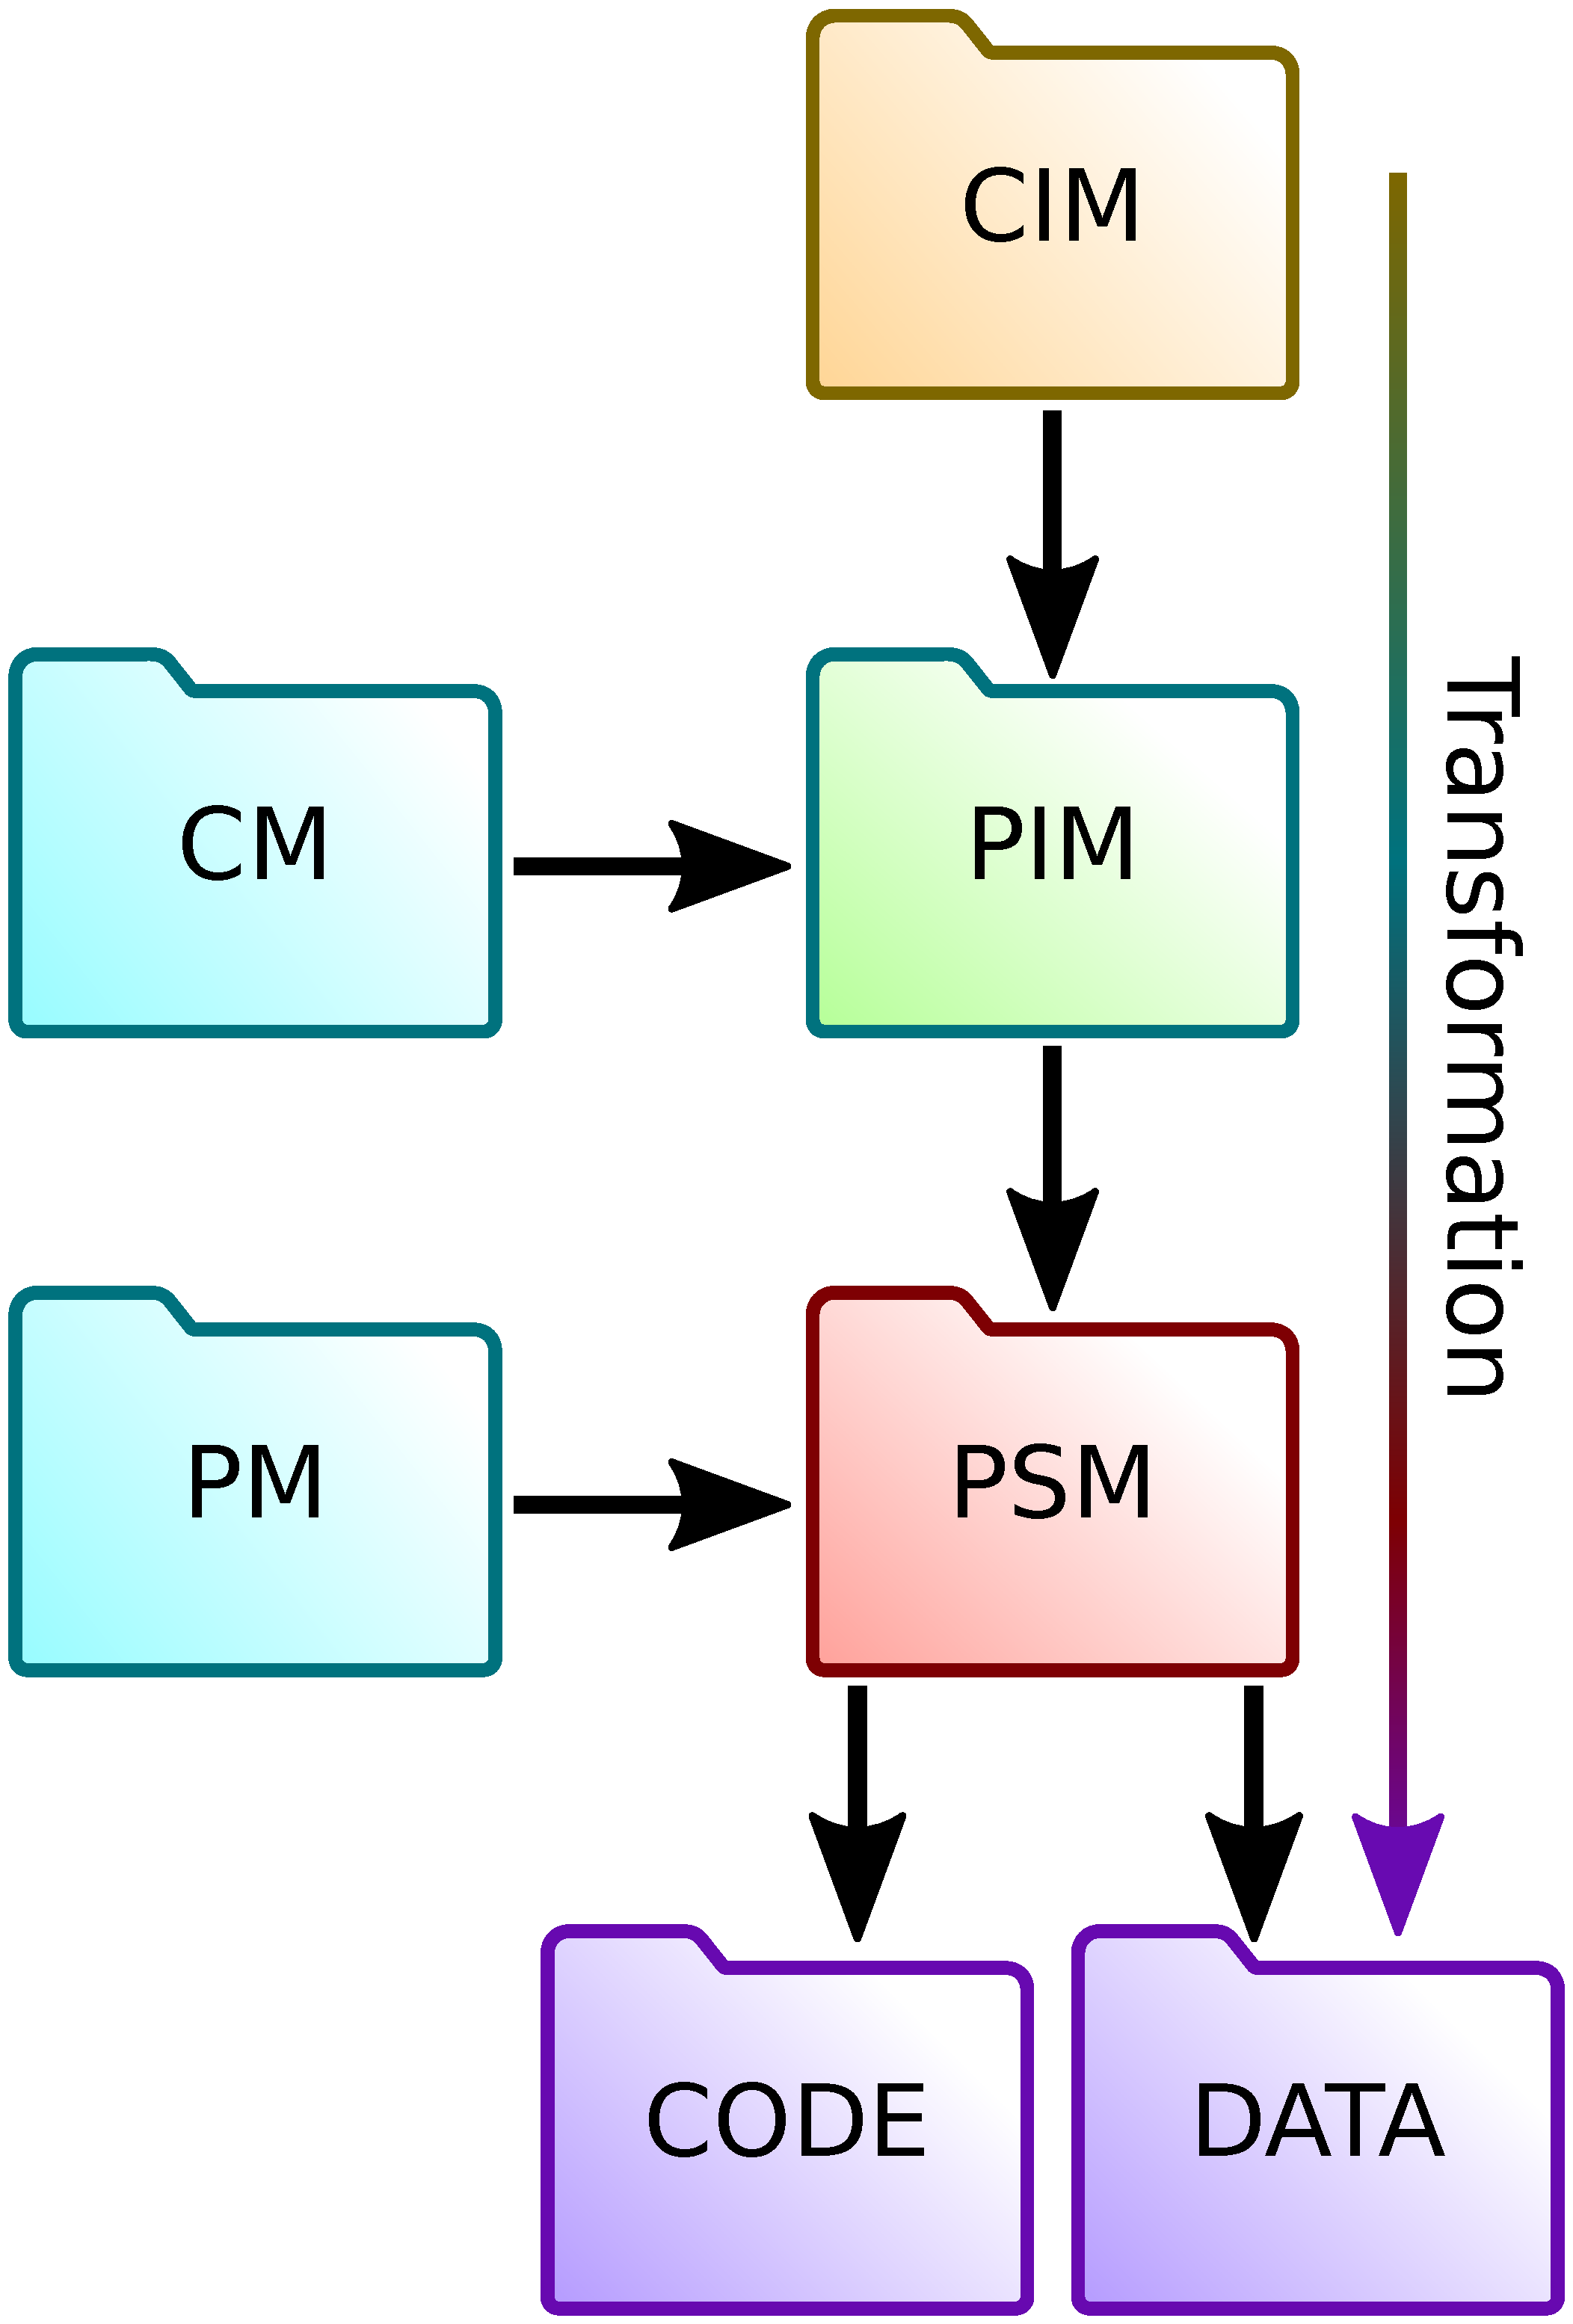
\includegraphics[width=1\linewidth]{mda-most-general.pdf}
    \end{column}
    \begin{column}{0.7\linewidth}
      \begin{description}
      \item[CIM] Computationally Independent Model;
      \item[CM] Model of Computations;
      \item[PIM] Platform Independent Model;
      \item[PM] Platform Model;
      \item[PSM] Platform--Specific Model;
      \item[CODE] Source code of software;
      \item[DATA] Initial database state.
      \end{description}
    \end{column}
  \end{columns}
\end{frame}

% \begin{frame}
%   \frametitle{Related technologies and standards}
%   \begin{itemize}
%   \item The most widely used technologies \textbf{ATL} and its predecessor QVT, an OMG standard; developed for XMI to XMI conversion;
%   \item Usage of ATL trending to shift to CIM level, \emph{e.g.}, BPMN diagram is converted into set of UML diagrams (PIM); used for construction web-applications, CIM is represented with State and Use case UML-Diagrams.
%   \item MDA usage is widening, \emph{e.g.}, for analysis of security aspects of distributed application with logical inference over MDA represented model;
%   \item UML is used as CIM/PIM in modeling vocabularies (ontologies); there is an OMG standard specification;
%   \item XML specifications are used to describe services, \emph{e.g.} WSDL, WS-BPEL;
%   \item MDA is opposed to conceptual programming by Enn Tyugu.
%   \end{itemize}

%   We describe transformation in Logtalk, representing CIM, PIM and PSM as RDF graphs, allowing non-XMI sources to be used, organizing multi-stage modular transformations.
% \end{frame}
\begin{frame}
  \frametitle{Logtalk as transformation definition language}
  We have chosen Logtalk as it
  \begin{itemize}
  \item inherits widely known Prolog language syntax and runtime;
  \item implemented as macro package, performance penalties are about 1.5\%;
  \item has flexible semantics: we can define transformations and constraints within the same syntax;
  \item implement object-oriented knowledge (rules) structuring, encapsulation and replacement;
  \item compositional way of transformation implementation;
  \item powerful engine to post constraints on object-to-object messages (events);
  \item has implementation for many Prolog engines.
  \end{itemize}
  The <<regular>> language allow us to use its libraries not directly related to MDA transformations.
\end{frame}
% \begin{frame}[fragile]
%   \frametitle{Semantic Web technologies in representation of models
%     during transformation}
%   \begin{itemize}
%   \item Assimilates experience of domain basic researches trending to standardization;
%   \item Regular set of triples denote a graph (T-Box, A-Box);
%   \item Standard vocabularies are formally described (\verb|rdfs:domain|, \verb|rdfs:range|);
%   \item Supported with most programming systems (libraries, inference engines, SPARQL);
%   \item RDF has a way of global element identification, \emph{i.e.} we can refer the same object from different software systems;
%   \item SWI-Prolog supports direct queries to a graph, as well as interpreting some predicates (\verb|rdfs:label|, \verb|dc:title|), wraps sparse RDF structure into a predicate arguments; ontological server ClioPatria;
%   \item There is simple way of data security implementation (\verb|rdfs:seeAlso|);
%   \item By means of Semantic Web \& LOD we are able to organize data transfer between heterogeneous information systems.
%   \end{itemize}
% \end{frame}

\begin{frame}
  \frametitle{Linked Open Data, LOD}
  \begin{enumerate}
  \item Information is published in Internet with open access license;
  \item It is represented in a machine-readable form, e.g., Excel table instead of a bitmap picture;
  \item An open format used, e.g., CSV instead of Excel;
  \item The format is based on W3C recommended standards, allowing RDF and SPARQL reference;
  \item Published data refer to objects, forming context.
  \end{enumerate}
  Thus, applications publish data as relations of objects (entities).
\end{frame}

\begin{frame}
  \frametitle{Model Driven Architecture and Linked Open Data}
  \begin{center}
    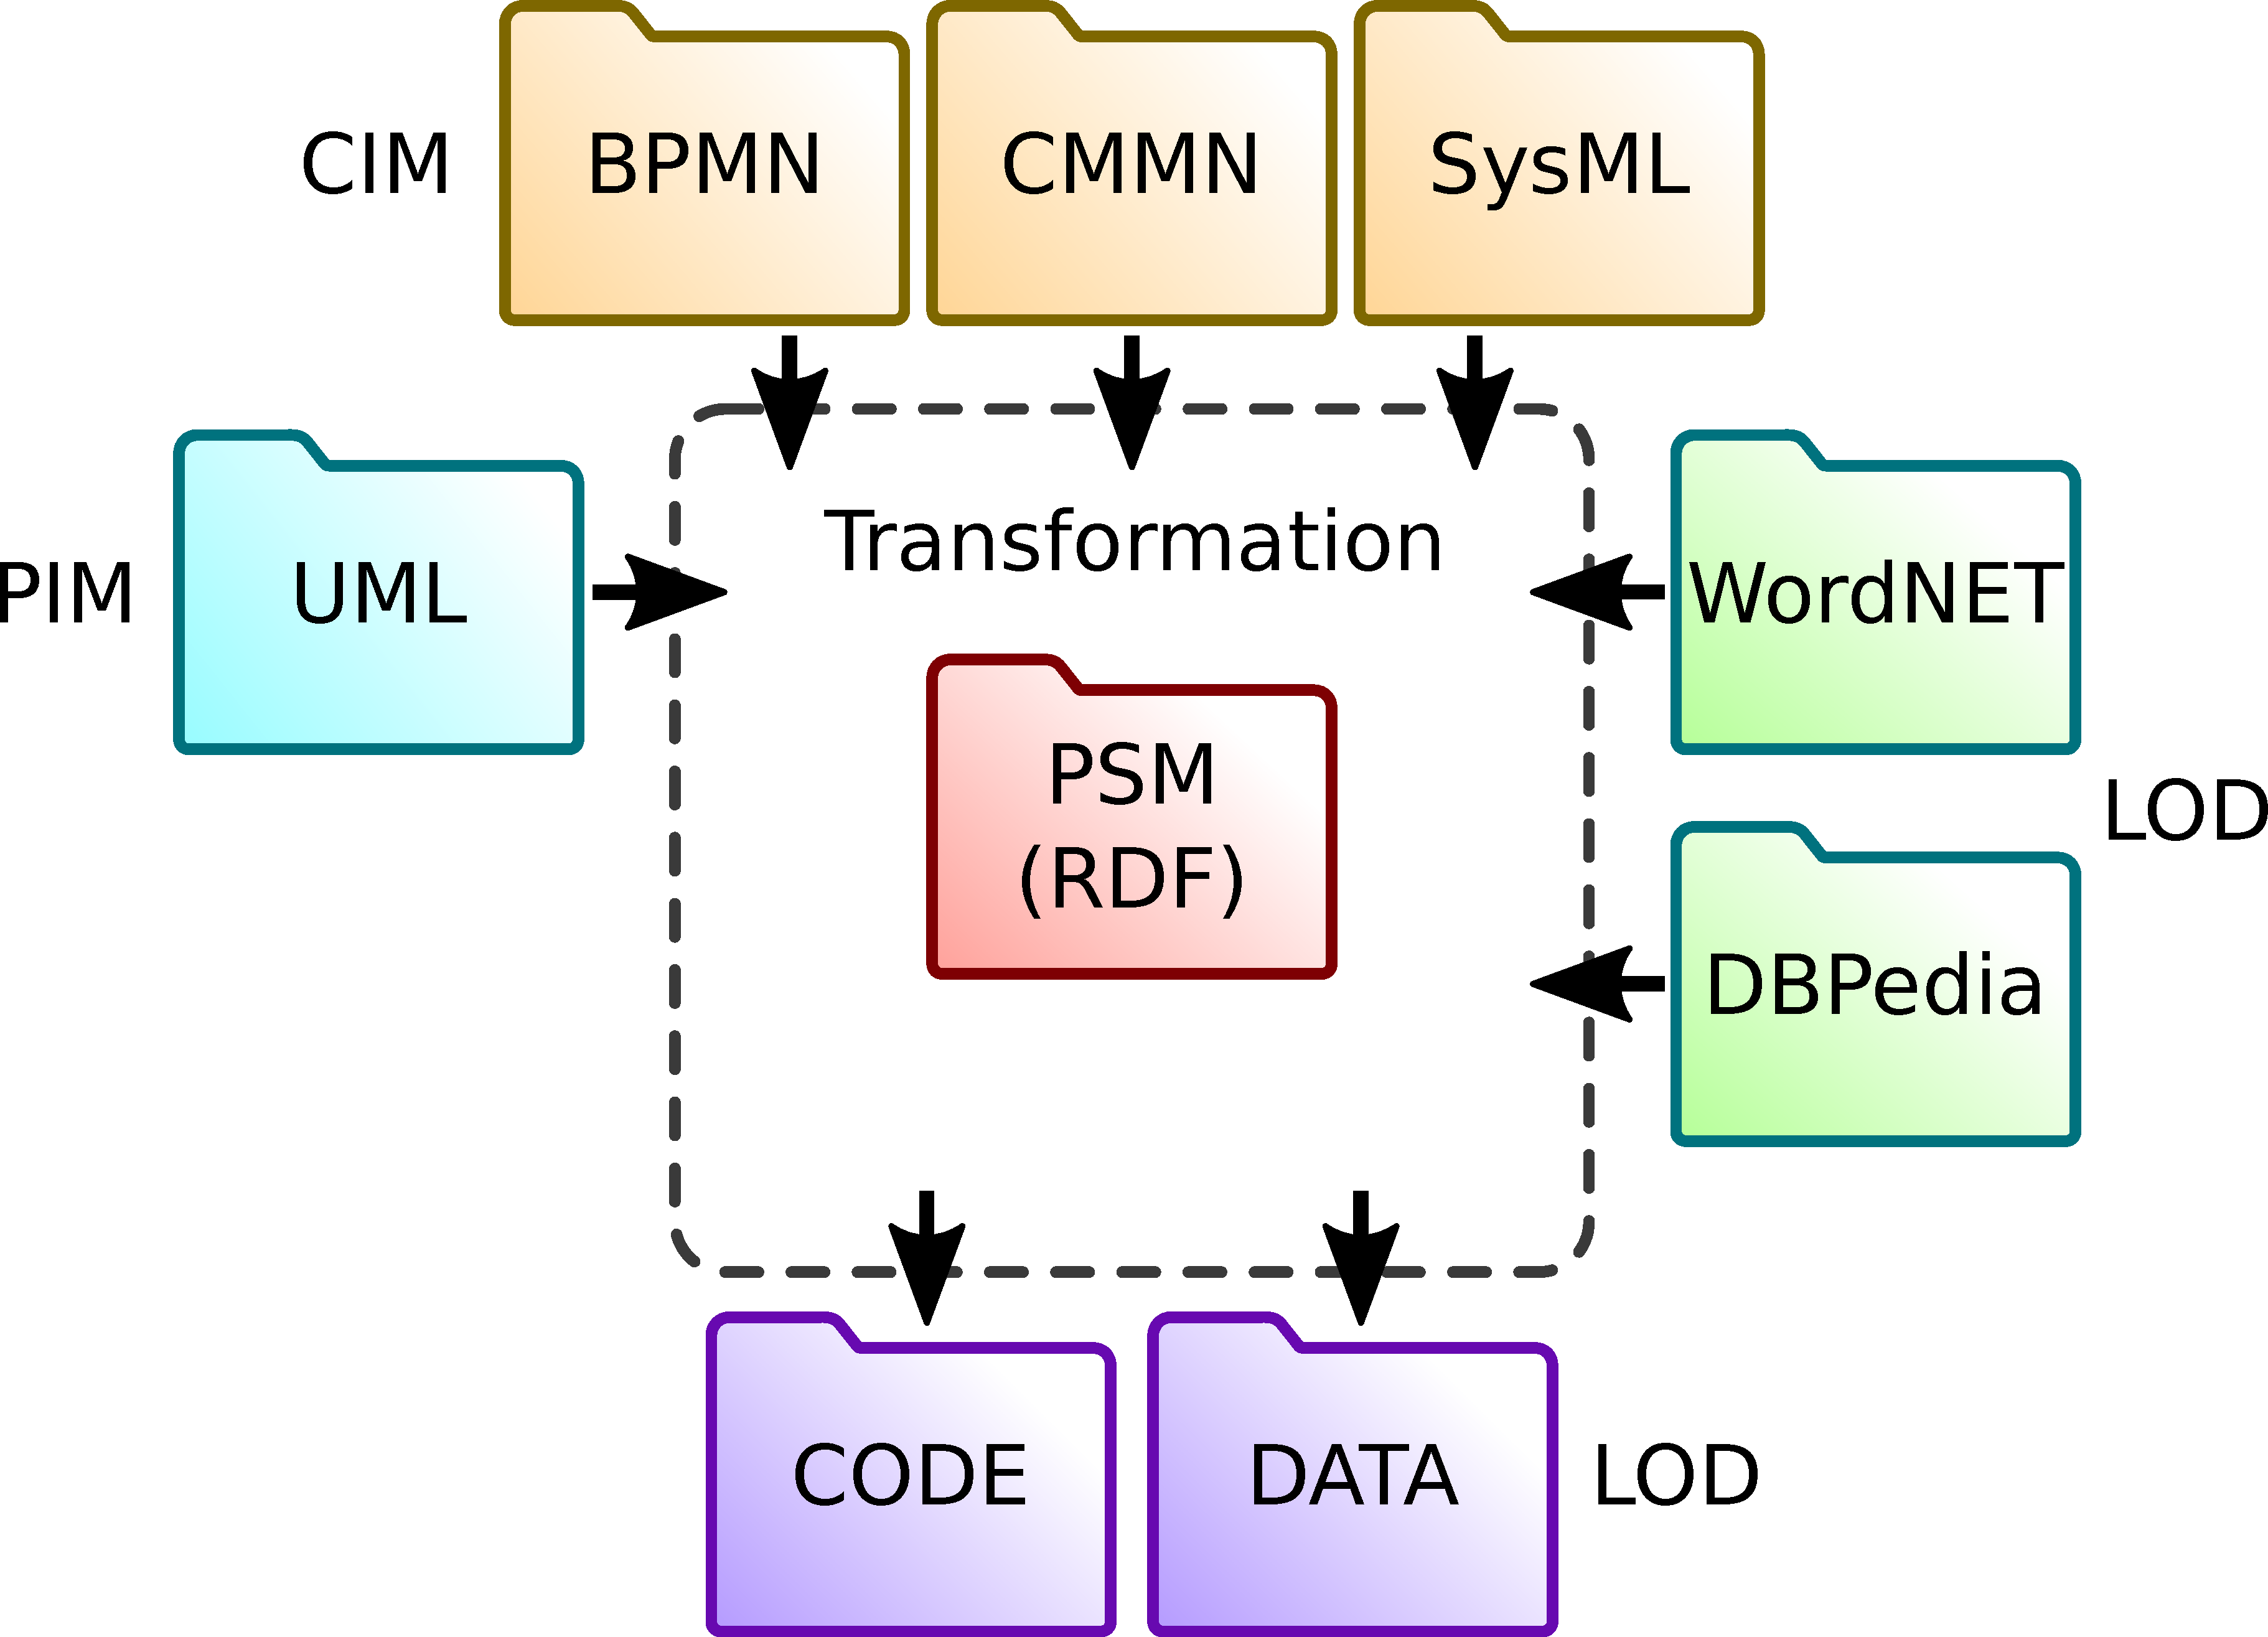
\includegraphics[width=0.9\linewidth]{mda-overview.pdf}
  \end{center}
\end{frame}
\begin{frame}
  \frametitle{MDA infrastructure}
  \centering
  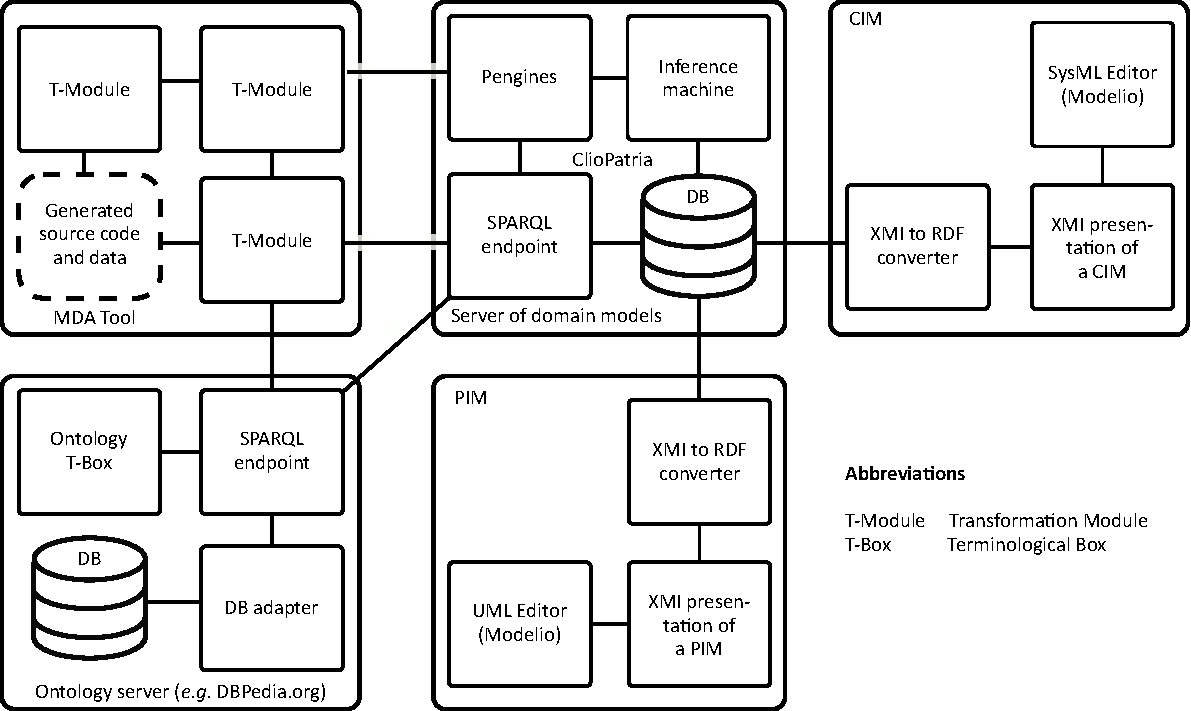
\includegraphics[width=1\linewidth]{architecture-mda-lod-ext.pdf}
\end{frame}
\begin{frame}
  \frametitle{Architecture of transformation modules}
  \centering
  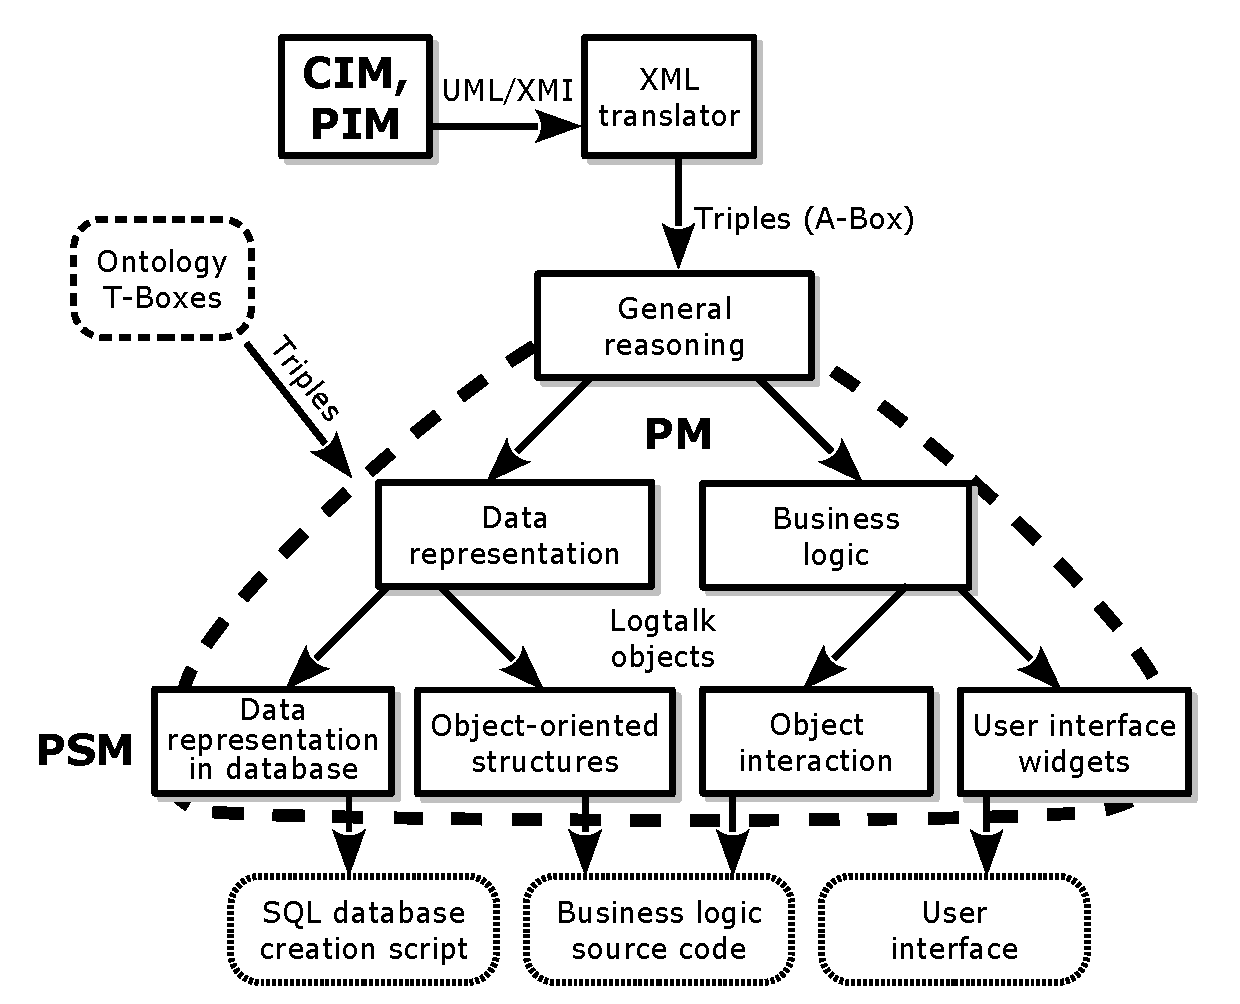
\includegraphics[width=0.9\linewidth]{architect_tree_pres-en-wo-OCL.pdf}
\end{frame}

\begin{frame}[fragile]
  \frametitle{PSM: Scenario of a Class synthesis}

%\begin{multicols}{2}
  \begin{columns}
    \begin{column}{0.6\textwidth}
\begin{minted}[fontsize=\tiny]{logtalk}
:- object(direct(_Package,_LocalProf,_CodeProf)).    % Transformation driver object
:- public([tr/4,tr/3]).                              % Public interface of a class synthesis scenario
% . . . . . . . . . .
tr(class, Class, ClassID):- ::package(Package),      % Synthesize a class
    query(Package)::class(Name, ClassID),            % Query package structure in XMI
    create_object(Class,      % . . . . .            % Create a <<Class>> object
    create_object(Attributes, % . . . . .            % Create <<Attributes>> object
    create_object(Methods,    % . . . . .            % ...<<Methods>>.
    Class::name(Name),                               % Name the class.
    % Generate attributes of the class,
    % organizing them in a local database.
    % ...methods...
    Class::attributes(Attributes),                   % Set the attributes for class.
    Class::methods(Methods).                         % ...methods.

tr(attribute, Attribute, ClassID, AttributeID):-     % Attribute transformations
    ::package(Package),
    query(Package)::attribute(Name,ClassID,AttrID),
    create_object(Attribute,  % . . . . .
    Attribute::name(Name).                           % Name the attribute.

tr(method, Method, ClassID, MethodID):-              % Transformation of methods
    ::package(Package),
    query(Package)::method(Name,ClassID,MethodID),
    create_object(Method,     % . . . . .
    Method::name(Name).                              % Name of the method
:- end_object.
\end{minted}
    \end{column}
    \begin{column}{0.4\linewidth}
      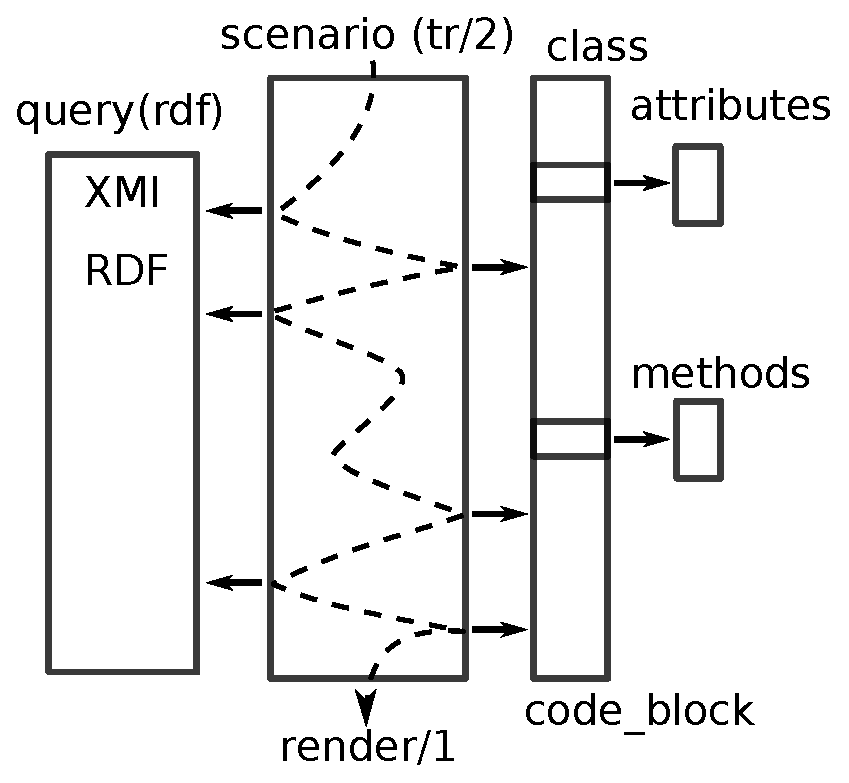
\includegraphics[width=1\linewidth]{scenario.pdf}
    \end{column}
  \end{columns}
  % \end{multicols}
\end{frame}

\begin{frame}[fragile]
  \frametitle{Implementation of \texttt{Query} object}
\begin{minted}[fontsize=\footnotesize{}]{logtalk}
:- object(query(_XMI)).
:- protected(xmi/1).
:- public([class/2, attribute/3, method/3]).
xmi(XMI) :- parameter(1, XMI).
class(Name, ID):-                            % Recognition of Class in RDF
    ::xmi(XMI),
    XMI::rdf(ID,rdf:type,uml:'Class'),
    XMI::rdf(ID,rdfs:label, literal(Name)).
attribute(Name, ClassID, ID):-               % ...attribute...
    ::xmi(XMI),
    XMI::rdf(ClassID, xmi:ownedAttribute, ID),
    XMI::rdf(ID, rdfs:label, literal(Name)).
method(Name, ClassID, ID):-                  % ...method...
    ::xmi(XMI),
    XMI::rdf(ClassID, xmi:ownedOperation, ID),
    XMI::rdf(ID, rdfs:label, literal(Name)).
% . . . . . . . . . . .
:- end_object.
\end{minted}
\end{frame}

\begin{frame}[fragile]
  \frametitle{Code Block (idea is taken from \texttt{llvmlite}${}^*$)}
  \begin{columns}
    \begin{column}{0.6\textwidth}
      \flushleft
\begin{minted}[fontsize=\footnotesize{}]{logtalk}
:- object(code_block, specializes(root)).
% Public interface of the object
:- public([append/1, prepend/1, clear/0,
   render/1, render_to/1, remove/1,
   item/1, items/1]).
% Code block items
:- dynamic([item_/1]).
:- private([item_/1]).
% Methods specialized during inheritance
:- protected([renderitem/2, render_to/2]).
% . . . . . . . . . . . .
% Delegate rendering to object itself
renderitem(Object, String):-
    current_object(Object), !,
    Object::render(String).
% Convert a literal to its string
% representation
renderitem(literal(Item), String):-!,
    atom_string(Item, String).
% Just print the item (debugging).
renderitem(Item, String):-
    root::iswritef(String, '%q', [Item]).
:- end_object.
\end{minted}
    \end{column}
    \begin{column}{0.4\textwidth}
      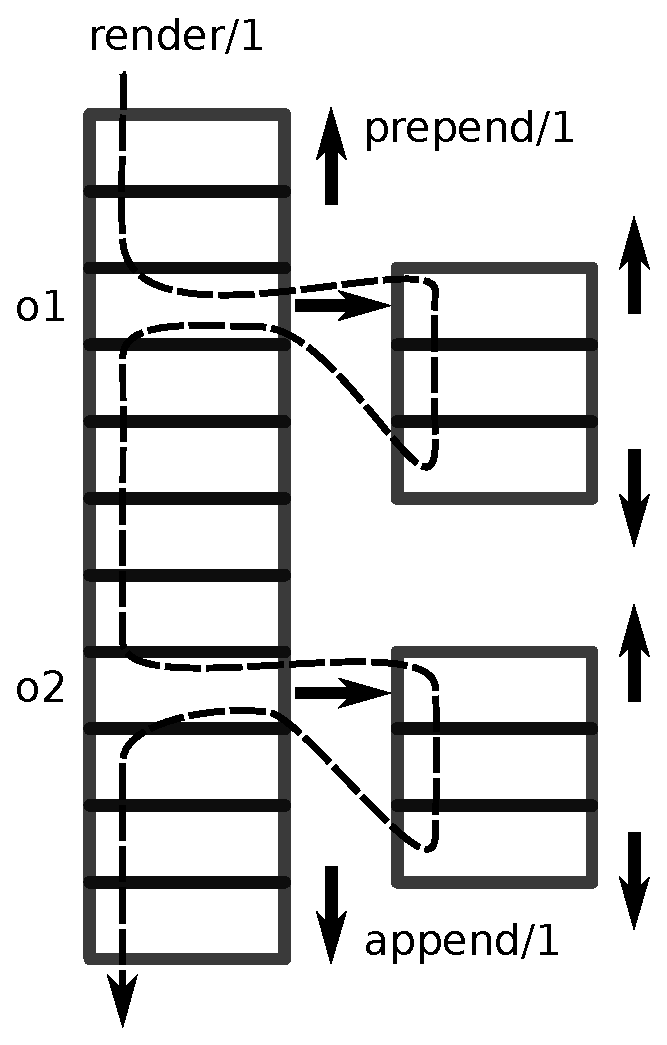
\includegraphics[width=1\linewidth]{code_block.pdf}
  ${}^*$) \url{https://github.com/numba/llvmlite}
    \end{column}
  \end{columns}
\end{frame}

\begin{frame}[fragile]
  \frametitle{PSM of a Python Class as a specialization of Code Block}
%\begin{multicols}{2}
  \begin{columns}
    \begin{column}{0.6\textwidth}
      \flushleft
\begin{minted}[fontsize=\scriptsize]{logtalk}
:- object(class, specializes(code_block),
   imports([named])). % Category of named entities
:- public([classlist/1, methods/1, attributes/1]).
% . . . . . . . . . . . . . .
renderitem(Item, Result):-      % proceed with default
    ^^renderitem(Item, Result). % rendering
render(Result):-         % Source generator
    ^^render(Name),      % implemented in a category
    ( ::item(classlist(List)) ->
     % . . . . . . . . . . .
        [Name]) ),
    ( ::item(attributes(Attributes))->
     % . . . . . . . . . . .
        [DefAttrList]),
      Attributes::items(InstanceAttrs),
      findall(S, ( % initialize attributes
         % . . . . . . . . .
         ), AttrAssigns),
        root::unindent,
        AttrList=[ConstructorDef|AttrAssigns];
         % . . . . . . . . .
        AttrList=[ConstructorDef, Pass] ),
    ( ::item(methods(Methods))-> % If any ...
      Methods::render(MethodList);
      MethodList=[] ),
    lists::append(AttrList,MethodList,StringList),
    root::unindent, Result=[Signature|StringList].
:- end_object.
\end{minted}
    \end{column}
    \begin{column}{0.4\linewidth}
      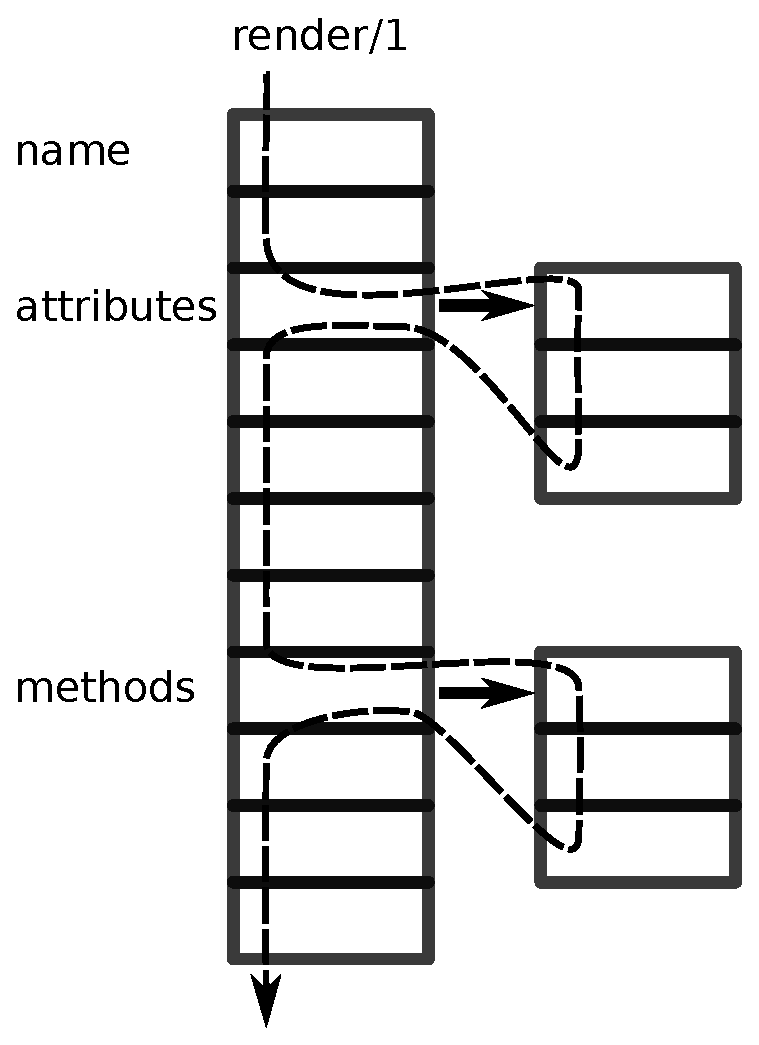
\includegraphics[width=1\linewidth]{code_block_class.pdf}
    \end{column}
  \end{columns}
  % \end{multicols}
\end{frame}

% \begin{frame}[fragile]
%   \frametitle{Logtalk Categories}
%   A category of named entities
% \begin{minted}[fontsize=\scriptsize]{logtalk}
% :- category(named).
% :- public([name/1, render/1]).
% :- protected([renderitem/2]).
% name(Name):- ::prepend(name(Name)).
% renderitem(name(Name), String):-!, atom_string(Name, String).
% render(String):-  % What is code generation from items
%     ::item(name(Name)), ::renderitem(name(Name), String).
% :-end_category.
% \end{minted}
% Category of named and typed entities
% \begin{minted}[fontsize=\scriptsize]{logtalk}
% :- category(namedtyped, extends(named)).
% :- public([type/1,render/2, separator_option/2,list_separator/1]).
% :- protected([renderitem/2]).
% type(Type):- ::append(type(Type)).
% renderitem(Item, String):- ^^renderitem(Item, String),!.
% renderitem(type(Type),String):-!, ::list_separator(Separator),
%     writef::swritef(String, '%w%w', [Separator, Type]).
% render(Middle, String):- ^^render(SName),
%     (   ::item(type(Type)) ->
%         ::renderitem(type(Type), SType),
%         string_concat(SName, Middle, _1),
%         string_concat(_1, SType, String) ;
%         SName = String  ).
% render(String):-  ::render("", String).
% list_separator(Separator):-
%     ::separator_option(Name, Default),!, % Global options
%     root::option(Name, Separator, Default).
% :- end_category.

% \end{minted}
% \end{frame}

% \begin{frame}[fragile]
%   \frametitle{Access LOD data}

%   \begin{columns}
% \begin{column}{0.5\textwidth}
% \begin{minted}[fontsize=\scriptsize]{logtalk}
% :- category(sparql).
% :- public(query/2).
% query(Pattern,Parameters,Row):-
%     prepare(Pattern,Parameters,Query),
%     server(Host,Port,Path),
%     sparql_query(Query, Row,
%         [host(Host),port(Port),path(Path)]).
% :- protected(server/3).  % must be implemented
%                          % by a subclass.
% :- protected(prepare/3). % prepares a query
% % . . . . . . . . . .    %             string.
% :- end_category.

% :- object(dbpedia, extends(sparql)).
% :- protected(server/3).
% server('dbpedia.org',80,'/sparql').
% :- public(entity_name/2).
% entity_name(Entity,Language,Name):-
%     query('select ?name where { '
%           ' %w rdfs:label ?name. '
%           'FILTER langMatches( lang(?label),'
%           ' "%w" )}', [Entity, Language],
%           row(Name)).
% :- end_object.

% % ?- dbpedia::entity_name(dbr:'Passport', 'ru', Name).
% \end{minted}
% \end{column}
% \begin{column}{0.5\textwidth}
%   \flushright
% 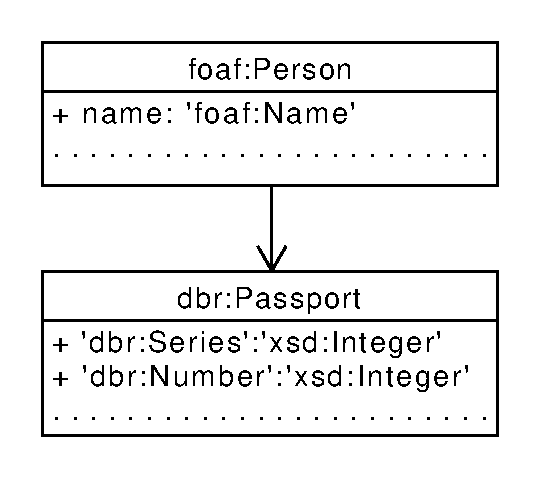
\includegraphics[width=0.8\linewidth]{simple-diag.pdf}
% \end{column}
% \end{columns}
% \end{frame}


\begin{frame}
  \frametitle{Applications: Dataflow representation of NGS analysis of amplicons}
  \begin{columns}
    \begin{column}{0.6\textwidth}
      \begin{raggedright}
        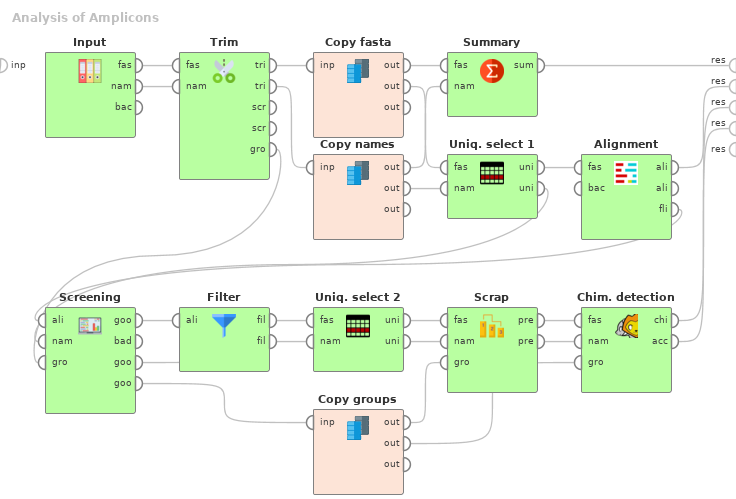
\includegraphics[width=1\linewidth]{Dataflow-color-en.png}
      \end{raggedright}
    \end{column}
    \begin{column}{0.4\textwidth}\footnotesize
      \begin{tabular}{ll}
        Term & Description \\
        \hline
        NGS & New Generation\\ & Sequencing\\
        Amplicon & A DNA or RNA part \\
                 & copied many times \\
        Mothur & A software toolset for\\ & NGS research \\
        Rapidminer & A visual tool for \\
             & data mining modeling\\
             &  and execution
      \end{tabular}
      ${}$\\[1em]
      Green blocks are Mothur modules. Others are Rapidminer modules.
    \end{column}
  \end{columns}
\end{frame}


\begin{frame}
  \frametitle{Discussion}
  Interesting positive impressions obtained:
  \begin{itemize}
  \item Logtalk and RDF are flexible, sufficiently universal and convenient implementation infrastructures for MDA;
  \item The best implemenation means is Prolog predicate wrapping and Logtalk object encapsulation of rules;
  \item Not all Logtalk properties are investigated: there might be more sophisticated programming techniques developed, \emph{e.g.}, on the base of message watchers.
  \end{itemize}
  Technical problems making the approach somewhat problematic:
  \begin{itemize}
  \item Very simple tasks take too much efforts, \emph{e.g.}, text processing: convert an identifier into the CamelCase;
  \item It takes too long to surf Internet in order to find a vocabulary for a domain, but it is more productive than development;
  \item Prolog is not a popular language in MDA, neither Logtalk.
  \end{itemize}
\end{frame}

\begin{frame}
  \frametitle{Application in developing KBS}
  Development and maintaining applied \textbf{knowledge--based systems (KBS)} in the up to date adequate state requires a lot of efforts devoted to solving problems of
  \begin{itemize}
  \item data model evolution,
  \item functionality expansion,
  \item graphical user interface modification.
\end{itemize}

To address these problems and, therefore, reduce the cost of creating, modifying and upgrading of applied KBS an automation of KBS development process is required.
\end{frame}

\begin{frame}
  \frametitle{Application in developing KBS}
  \begin{center}
  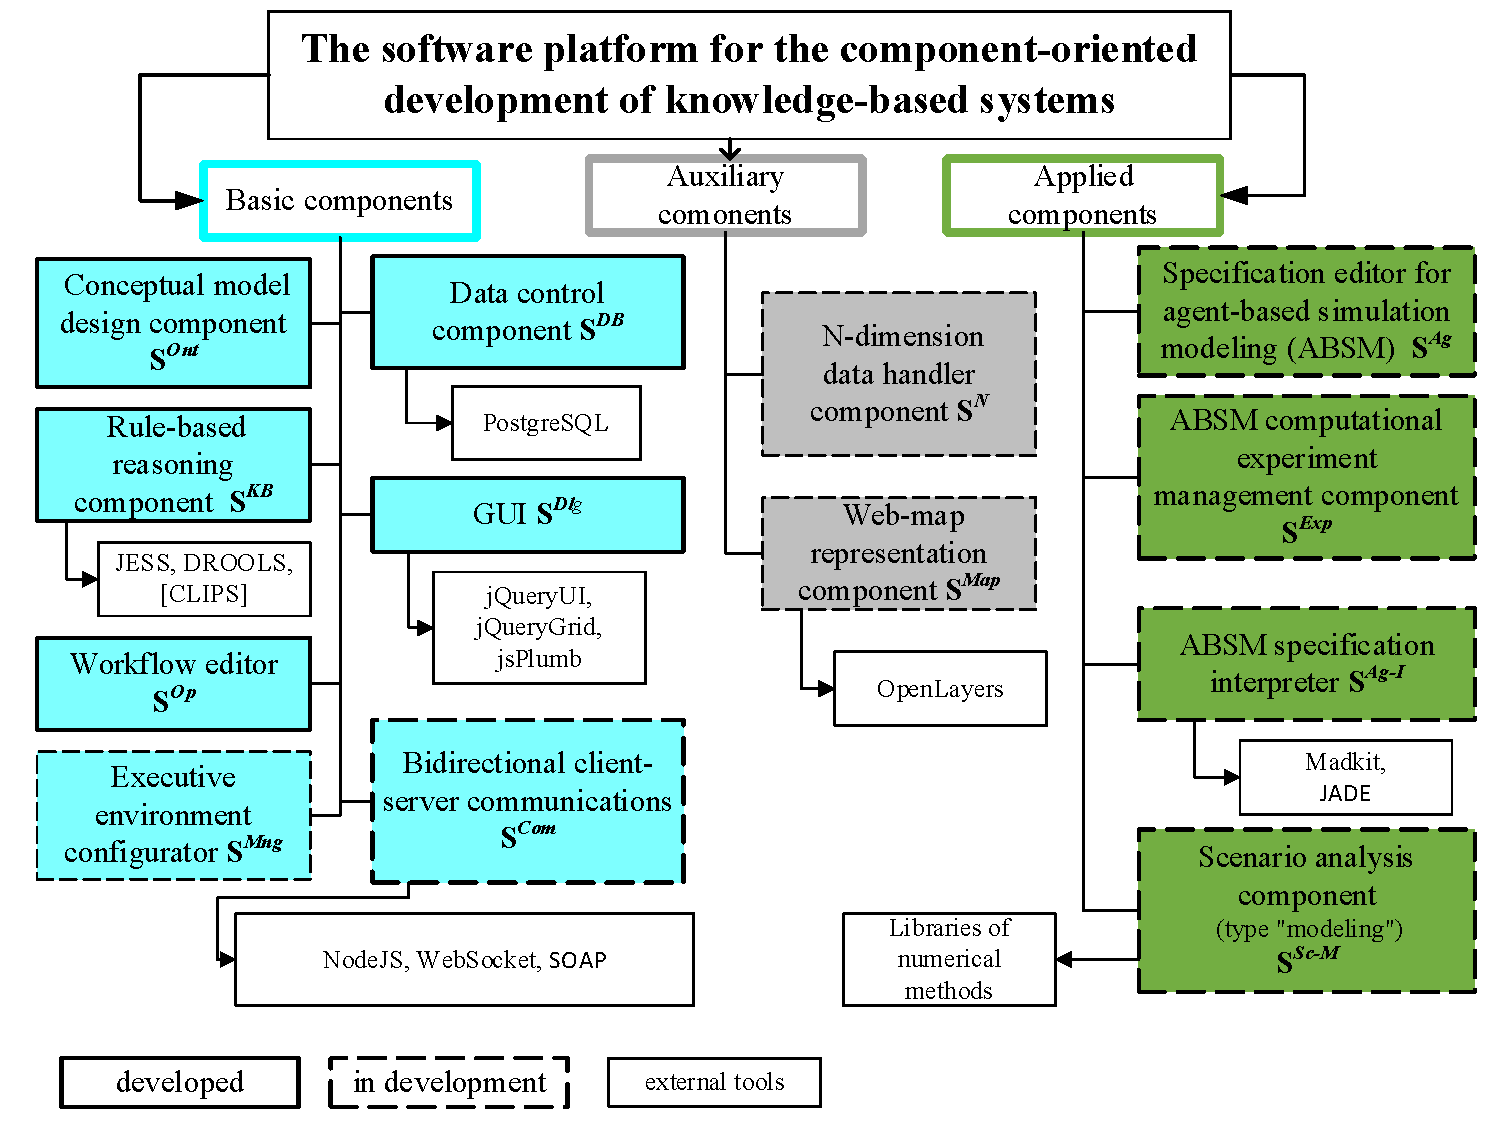
\includegraphics[width=0.9\linewidth]{kbs-stolboff.pdf}
\end{center}
\end{frame}

\begin{frame}
  \frametitle{Document authoring and storage}
  In most cases documents are created as a result of
  \begin{itemize}
  \item creative activity of a person with a text processors (authoring);
  \item printing a digital copy or a data record in a database;
  \item aggregation operation over database records (report).
  \end{itemize}
  Then it is stored either as a physical paper and/or a digital document (PDF, DOCX, HTML).

  Since 2000-th, Semantic Web and Linked Open Data (LOD) is being developed, allowing
  \begin{itemize}
  \item structural storage of data within published documents;
  \item processing stored data computationally;
  \item integration of data structures and data objects globally.
  \end{itemize}

  The \textbf{aim of this research} is to develop technologies, software and services allowing construction of digital archives supporting document data inclusion and inference from existing documents.
\end{frame}

\begin{frame}
  \frametitle{Structure of a document}
  \centering
  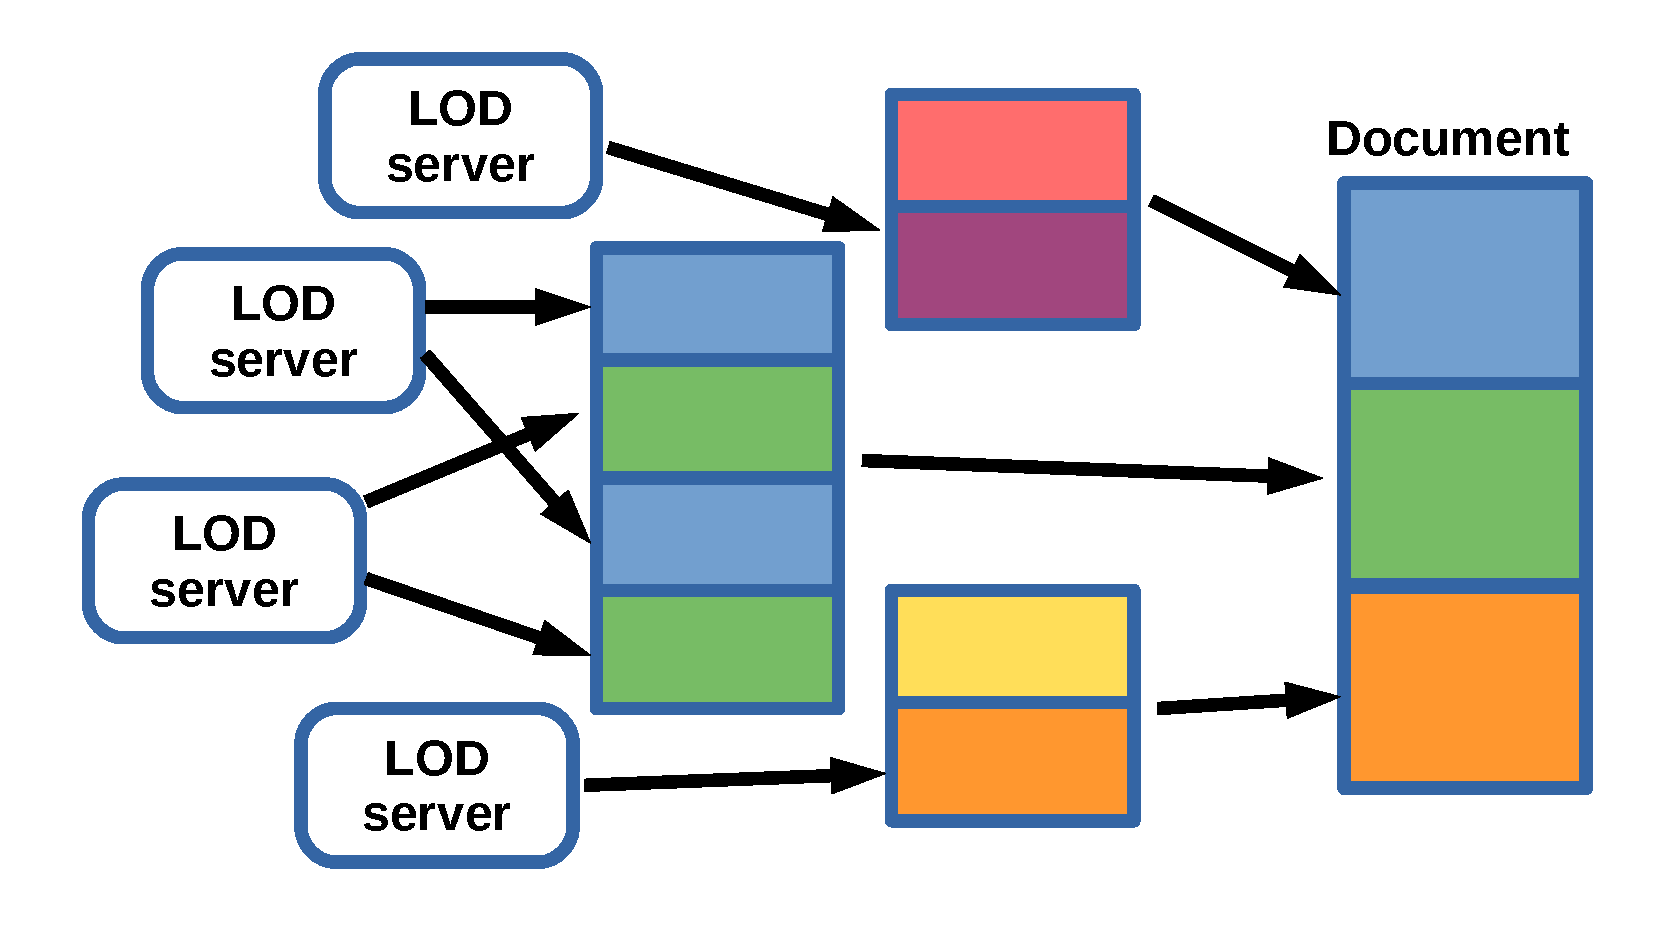
\includegraphics[width=1\linewidth]{document-structural-view.pdf}
\end{frame}

\begin{frame}
  \frametitle{Open Annotaiton (oa)}
\begin{adjustwidth}{-3em}{-3em}
  \centering
  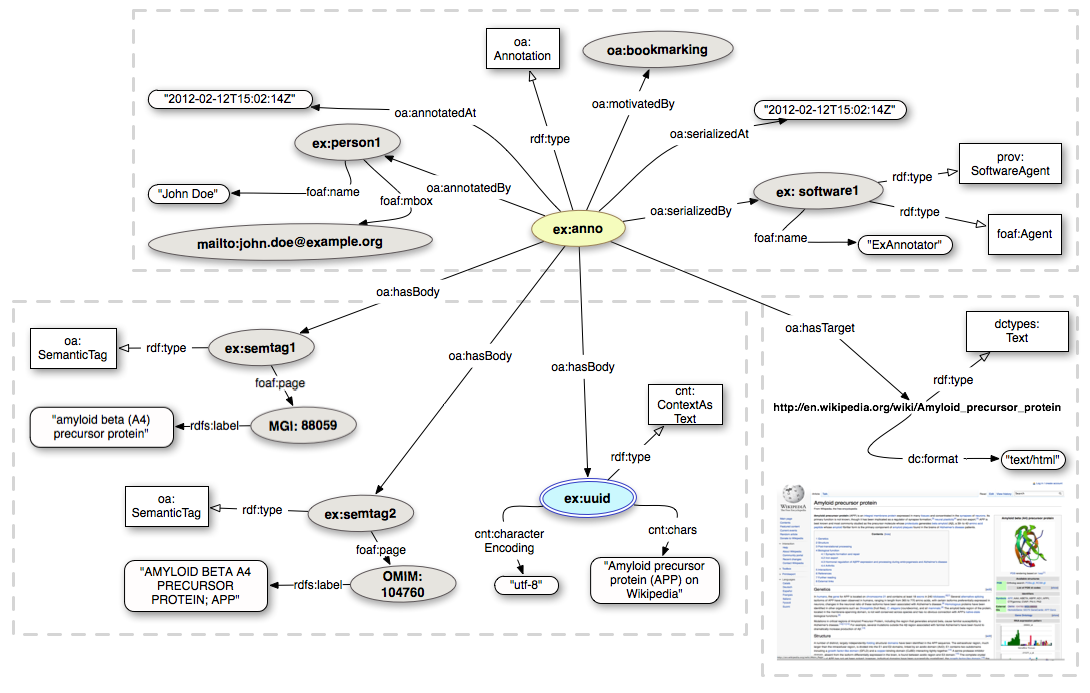
\includegraphics[width=1\linewidth]{Open-Annotation_CB_Bookmarking_and_Semantically_Tagging_A_webpage_spec20130128.png}
\end{adjustwidth}

\end{frame}

\begin{frame}[fragile,fragile]
  \frametitle{Representation}
  % \begin{block}{}
  %   \textbf{Целью} исследования является создание методики разработки процедур трансформации (PD\footnote{Platform [description] model.}) в виде ОО-модулей.
  % \end{block}
  % \begin{columns}
  %   \begin{column}{0.5\linewidth}
  %     % 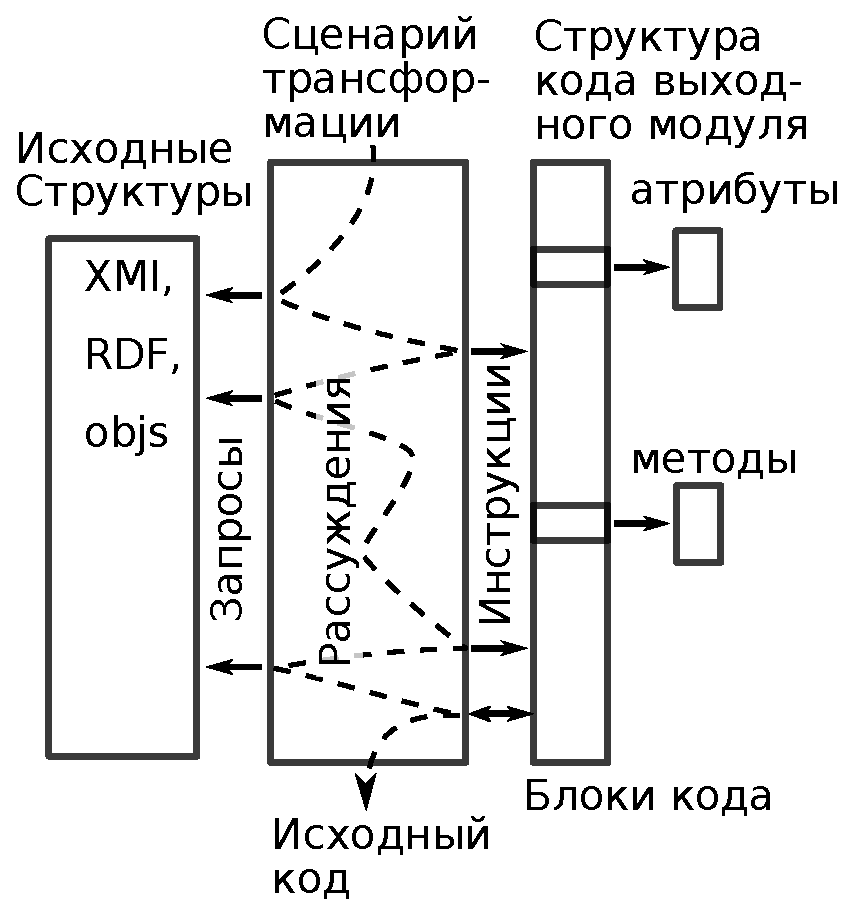
\includegraphics[width=1\linewidth]{pics/scenario-ru-wo-mothur.pdf}
  %   \end{column}
  %   \begin{column}{0.6\linewidth}
  %     Задачи исследования:
  %     \begin{itemize}
  %     \item Изучить синтаксические структуры Logtalk в аспекте структурирования знаний;
  %     \item Предложить методику представления трансформации в виде ОО-модулей;
  %     \item Реализовать библиотеку объектов и классов для МДА;
  %     \item Тестирование библиотеки на примере.
  %     \end{itemize}
  %   \end{column}
  % \end{columns}

\begin{adjustwidth}{-1.5em}{-1.5em}
\begin{minted}[escapeinside=||,fontsize=\btprgsize]{xml}
<html lang="ru" xmlns=http://www.w3.org/1999/xhtml
|\GB{xmlns:taa}|=http://irnok.net/engine/rdfa-manipulation
xml:lang="ru" metal:define-macro="page">
<head> . . . . </head>
<body prefix="rdf: http://www.w3.org/1999/...-ns# foaf: http://xmlns.com/foaf/...
imei: imei.html# course: https://irnok.net/college/plan/01..16-...\
%D0\%BA_PB-SM.plm.xml.xlsx-....2.3.1.html#"  resource="#post"
typeof="schema:CreativeWork sioc:Post prov:Entity">
<!-- The application control panel -->

<main lang="ru" resource="#annotation" typeof="oa:Annotation" id="main-doc-cnt">
<div property="oa:hasTarget" resource="#course-work-prog"></div>
<article property="oa:hasBody" typeof="foaf:Document curr:WorkingProgram"
         resource="#course-work-program" id="main-document">
  <div |\GB{taa:content}|="imei:title-page"></div>
  <div |\GB{taa:content}|="imei:neg-UMK"></div>
  <section id="TOC" class="break-after"> <h2>Table of Contents</h2>
    <div id="tableOfContents"></div>
  </section>
  <section id="course-description" resource="#description"
           property="schema:hasPart" typeof="schema:CreativeWork">
    <div property="schema:hasPart" resource="#purpose"
         typeof="dc:Text cnt:ContentAsText" >
      <div property="cnt:chars" datatype="xsd:string">
        <h2 property="dc:title" datatype="xsd:string">
           Aims and objectives of the discipline (module)</h2>
        <p>The aim of teaching the discipline ...</p>
      </div>
   </div>
  . . . . . . . .
\end{minted}
\end{adjustwidth}
\end{frame}

\begin{frame}
  \frametitle{Architecture}
  \begin{adjustwidth}{-2.5em}{-2.5em}
    \begin{center}
      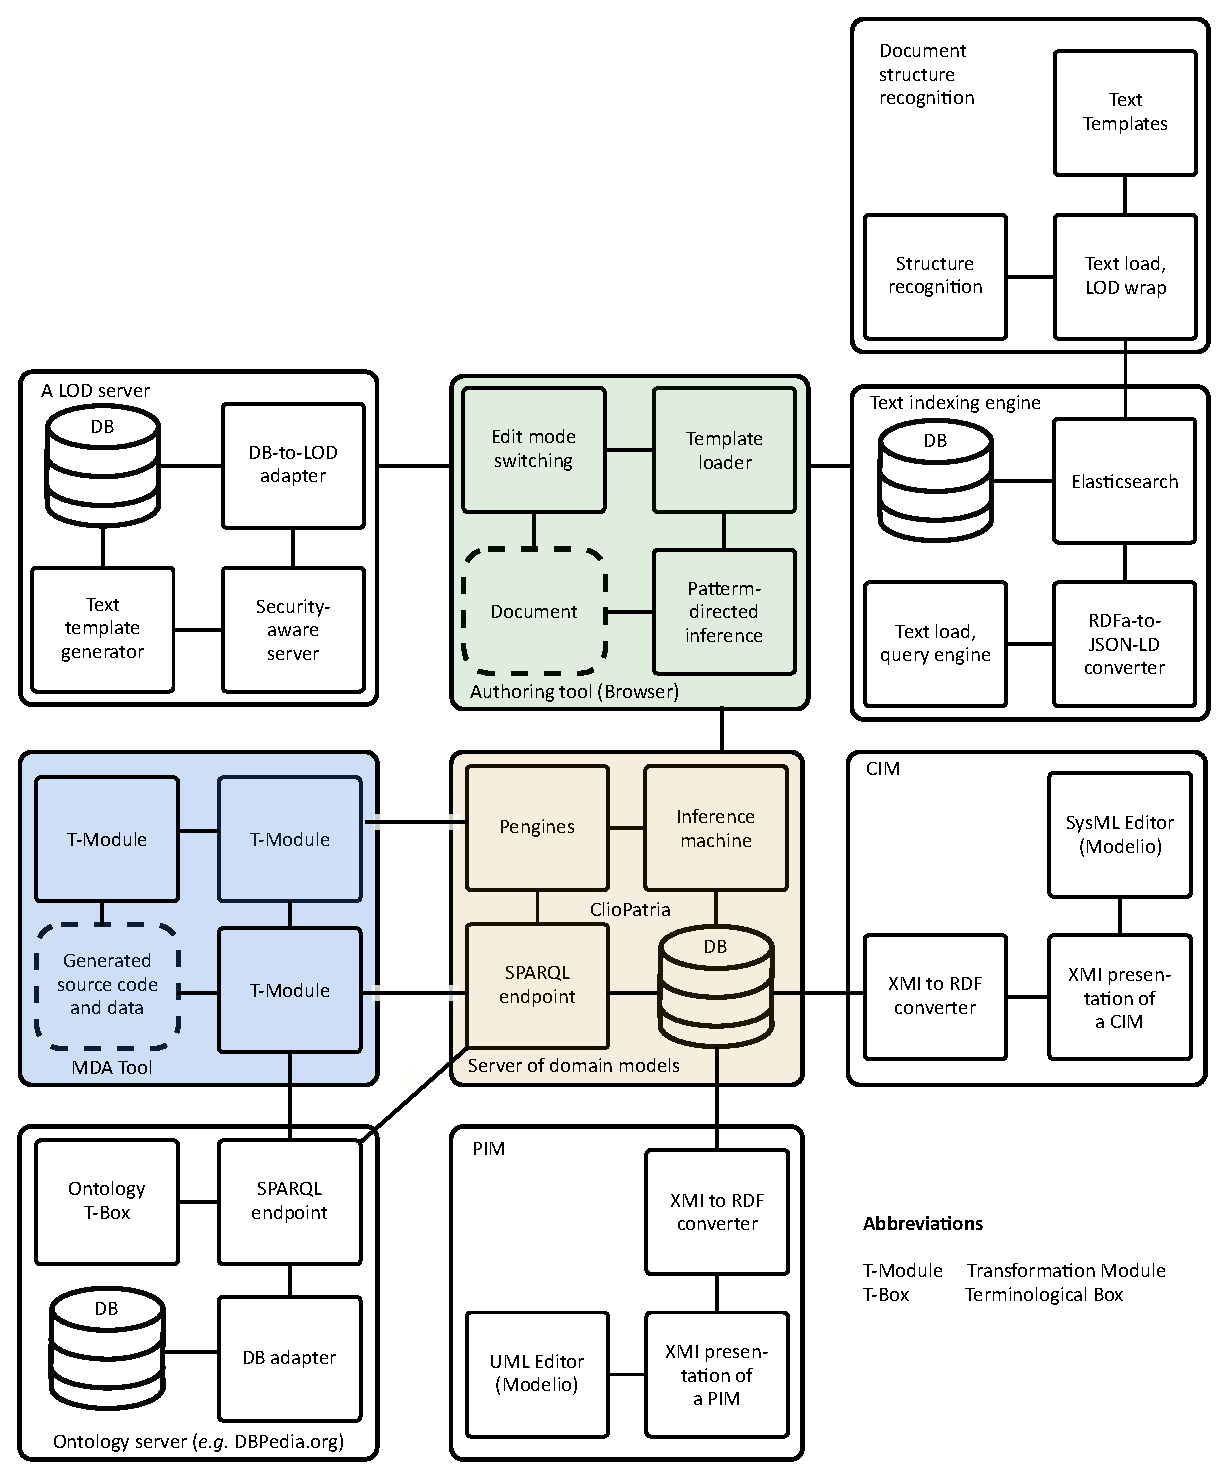
\includegraphics[width=0.5\linewidth]{architecture-mda-lod-ext-tot.pdf}
    \end{center}
  \end{adjustwidth}

% \begin{itemize}
% \item content and metadata repository with SPARQL (6) and full-text search (3); the engines for LOD processing (5) based on the logical inference;
% \item service for analysis of the stored content (2) enriching the archive with semantic information describing the content;
% \item tools for development of LOD applications and their user interfaces (1);
% \item browser based authoring tools (4).
% \end{itemize}
\end{frame}

\begin{frame}
  \frametitle{Generated list of title page preambles}
    \begin{adjustwidth}{-2.5em}{-2.5em}
    \begin{center}
      
\includegraphics[width=0.7\linewidth]{template-title-pages.jpg}
    \end{center}
  \end{adjustwidth}
\end{frame}

\begin{frame}
  \frametitle{Generated part of a study program}
   \begin{adjustwidth}{-2.5em}{-2.5em}
    \begin{center}
      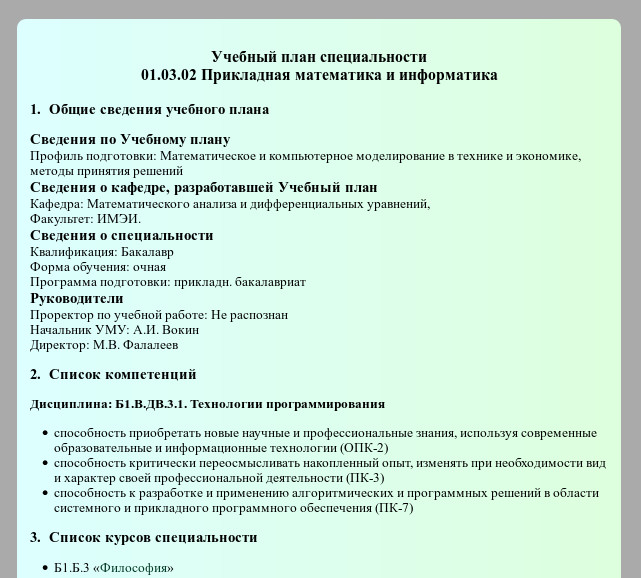
\includegraphics[width=0.7\linewidth]{template-courses.jpg}
    \end{center}
  \end{adjustwidth}
\end{frame}
\begin{frame}
  \frametitle{Imported time distribution for lecture, seminary, \ldots}
   \begin{adjustwidth}{-2.5em}{-2.5em}
    \begin{center}
      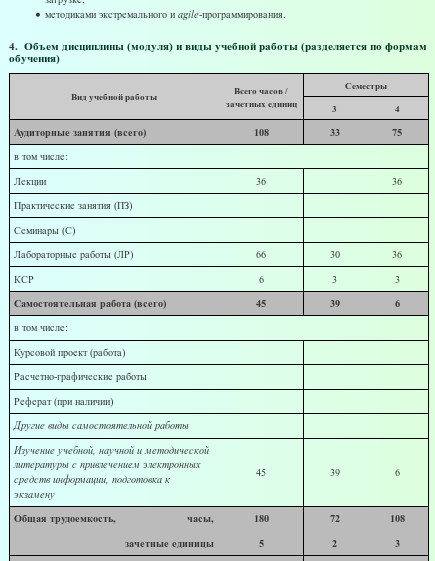
\includegraphics[width=0.9\linewidth]{work-program-volume.jpg}
    \end{center}
  \end{adjustwidth}
\end{frame}

\begin{frame}
  \frametitle{Complete document}
  \begin{adjustwidth}{-2.5em}{-2.5em}
    \begin{center}
      \begin{columns}
        \begin{column}{0.5\linewidth}
          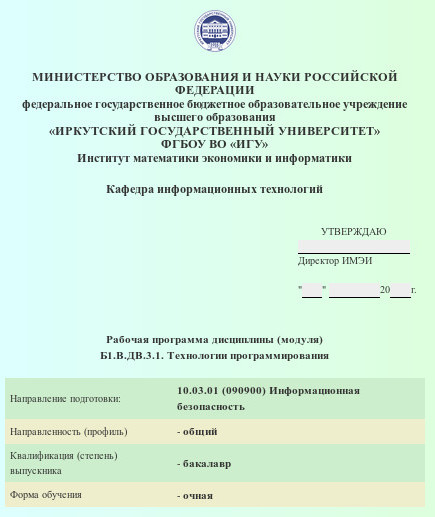
\includegraphics[width=1\linewidth]{work-program-title.jpg}
        \end{column}
        \begin{column}{0.5\linewidth}
          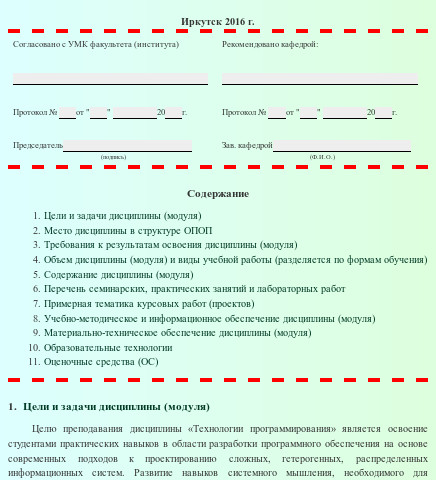
\includegraphics[width=1\linewidth]{work-program-agreement.jpg}
        \end{column}
    \end{columns}
    \end{center}
  \end{adjustwidth}
\end{frame}

\begin{frame}
  \frametitle{Used ontologies}
  \begin{itemize}
  \item Friend-of-a-friend (\textbf{foaf}) - agent information: individuals, legal entities, program agents.
  \item Provenance (\textbf{prov}) - references between documents.
  \item Dublin Core (\textbf{dc}) - edited annotation mark up.
  \item DBPedia resource (\textbf{dbr}) – references to instant objects and classes.
  \item Schema.org (\textbf{schema}) - Google, Yandex, Yahoo, \emph{etc}. searchable objects, structural elements.
  \item The Bibliographic Ontology (\textbf{bibo}) - literature reference mark up.
\end{itemize}
\end{frame}

\begin{frame}
  \frametitle{Conclusion}
A tools (components) for digital archive implementation, which allows
to device information systems and document processing services
with the following features:
\begin{itemize}
\item load LOD marked up document, extract, store in a graph and index RDF data;
\item retrieve RDF data as triples or as a result of full-text search query;
\item combine existing LOD data and its content in new documents dynamically with browser based context inference machine;
\item use server-site inference machine (Prolog) to process RDF data upon
  request from browser's part of the system;
  % \item organizes a platform for document semantic markup,
\item convert created RDFa marked up HTML5 documents into Excel and Word formats.
\end{itemize}

  \textbf{Applications}
  \begin{itemize}
  \item Document authoring automation;
  \item Context-depended editing;
  % \item Export into office formats;
  \item Self-organizing global document flows;
  \item Documents as data sources for information systems.
  \end{itemize}

\end{frame}

% \begin{frame}
%   \frametitle{Conclusion}
%   The following results have been obtained as for today:
%   \begin{itemize}
%   \item A technique for model representation has been developed and tested.
%   \item A programming technique using object-oriented logical language Logtalk is deviced.
%   \item Ptototypes of various transformation procedures are implemented.
%   \item Transformation tools are tested in application areas and no significant technical problems were mentioned.
%   \end{itemize}
%   Further development directions are as follows:
%   \begin{itemize}
%   \item A technique for document automatic markup with vocabulary entities.
%   \item A transformation implemenation techniques, minimizing usage of dynamic objects, targeting on macro properties of Logtalk.
%   \item Form a toolset out of existing prototypes obeing nowadays software development requirements.
%   \end{itemize}
%   The source codes are available at \url{https://github.com/isu-enterprise/icc.xmitransform}, \url{https://github.com/eugeneai/icc.mothurpim}.
% \end{frame}



\begin{frame}
  \frametitle{Tabby{XL}}
  \vfill
  \begin{center}
    {\bfseries Software Platform for Rule-Based Spreadsheet Data Extraction and Transformation}\\
    \medskip
     Alexey Shigarov, Vasiliy Khristyuk, et al\\
    \medskip
    \texttt{shigarov@icc.ru} % Your email address
  \end{center}
  \vfill
\end{frame}

\begin{frame}
\frametitle{Motivation}
\begin{itemize}
\item About arbitrary spreadsheet tables
\begin{itemize}
	\item A large volume of valuable data for science and business applications
	\item A big variety of layout, style, and content features
	\item Human-centeredness (incorrect structure and messy content)
	\item No explicit semantics for interpretation by computers
\end{itemize}
\bigskip
\item Challenges
\begin{itemize}
	\item How to extract tables from worksheets
	\item How to recognize and correct cell structure anomalies
	\item How to recover semantics needed for the automatic interpretation
	\item How to conceptualize extracted data by using external vocabularies
\end{itemize}
\end{itemize}
\end{frame}

\begin{frame}
\frametitle{Background}
\emph{Table understanding} includes the following tasks
\bigskip
\begin{enumerate}
	\item \textbf{Extraction} --- detecting a table and recognizing the physical structure of its cells
	\item \textbf{Role analysis} --- extracting functional data items from cell content
	\item \textbf{Structural analysis} --- recovering internal relationships between extracted functional data items
	\item \textbf{Interpretation} --- linking extracted functional data items with external vocabularies (general-purpose or domain-specific ontologies)
\end{enumerate}
\end{frame}

% \begin{frame}
% \frametitle{Background}
% The related issues of the \emph{table analysis and interpretation}
% \bigskip
% {\footnotesize
% \begin{itemize}
% \item \textbf{Layout properties} \cite{Koci2017,Chen2017,Dou2018}
% \item \textbf{Code smells and formulas} \cite{Hermans2015,Dou2017,Barowy2018,Koch2019}
% \item \textbf{Programming by examples} \cite{Barowy2015,Singh2016,Jin2017}
% \item \textbf{Data model inference} \cite{Amalfitano2015,Cunha2015,Cunha2016}
% \item \textbf{Linked Open Data} \cite{Ritze2017,Zhang2017}
% \item \textbf{Domain-specific models} \cite{Vos2017,Cao2017,Swidan2017}
% \item \textbf{Rule-based programming} \cite{Yang2017,Shigarov2017,Yang2018}
% \end{itemize}
% }
% \end{frame}

% \begin{frame}
% \frametitle{Background}
% The projects with goals similar to ours
% \bigskip

% \begin{enumerate}
% \item \footnotesize{\textbf{TANGO}\footnote{\url{https://tango.byu.edu}} (Data Extraction Group, Brigham Young University) \textit{2005 -- 2016}}
% \begin{itemize}
% \item \scriptsize{Heuristics-based role analysis (pre-defined functional cell regions) \cite{Embley2016}}
% \end{itemize}
% \item \footnotesize{\textbf{Senbazuru}\footnote{\url{http://dbgroup.eecs.umich.edu/project/sheets}} (Database Research Group, University of Michigan) \textit{2013 -- 2017}}
% \begin{itemize}
% \item \scriptsize{ML-based role analysis (pre-defined functional cell regions) \cite{Chen2016}}
% \item \scriptsize{ML-based structural analysis (pre-defined layout properties of the header hierarchy) \cite{Chen2016}}
% \end{itemize}
% \item \footnotesize{\textbf{DeExcelerator}\footnote{\url{https://wwwdb.inf.tu-dresden.de/research-projects/deexcelarator}} (Dresden Database Systems Group, TU Dresden) \textit{2013 -- 2019}}
% \begin{itemize}
% \item \scriptsize{ML-based layout identification}~\cite{Koci2016}
% \item \scriptsize{Heuristics-based role and structural analysis (pre-defined functional cell regions) \cite{Koci2017,Koci2018}}
% \end{itemize}
% \end{enumerate}

% \end{frame}


% \subsection{Contribution}

\begin{frame}
\frametitle{Contribution}
\small TabbyXL is a software platform aiming at the development and execution of rule-based programs for spreadsheet data extraction and transformation from arbitrary (\textit{a}) to relational tables (\textit{b})
\begin{columns}[c] % The "c" option specifies centered vertical alignment while the "t" option is used for top vertical alignment
\column{.4\textwidth} % Left column and width
\begin{block}{\small Novelty}
\begin{itemize}
\item \small Table object model assigning roles to data items, not cell
\item \small CRL, domain-specific language to express user-defined rules for table analysis and interpretation
\item \small CRL-to-Java translator to synthesize executable programs for spreadsheet data transformation
\end{itemize}
\end{block}
\column{.6\textwidth} % Right column and width
%\begin{figure}
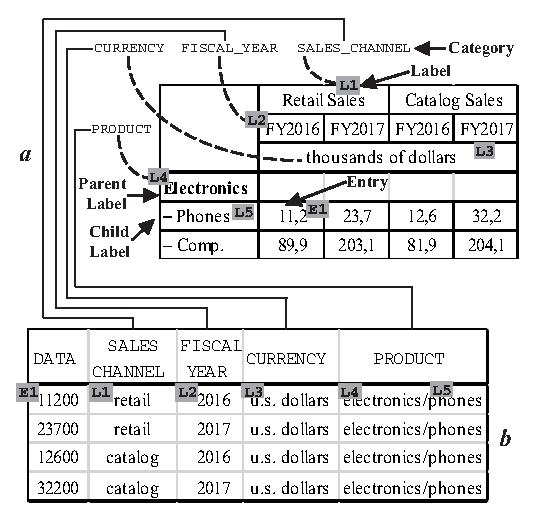
\includegraphics[width=0.85\linewidth]{intro}
%\end{figure}
\end{columns}
\end{frame}

% \section{Approach}

%\subsection{User-Defined Rules}

% \begin{frame}
% \frametitle{User-Defined Rules}
% \begin{itemize}
% \item The user-defined rules map the physical structure into the logical structure of a table
% \begin{itemize}
% \item \textbf{WHEN-part} queries facts about the structure by using constraints
% \item \textbf{THEN-part} modifies available facts and asserted new ones
% \end{itemize}
% \item The facts are represented by items of the \emph{table object model}
% \item The rules can be expressed in a rule-based language
% (e.g. Drools\footnote{\url{https://www.drools.org}}, Jess\footnote{\url{https://jessrules.com}}, or CRL\footnote{\url{https://github.com/tabbydoc/tabbyxl/wiki/crl-language}})
% \end{itemize}
% \end{frame}

% \subsection{Table Object Model}

\begin{frame}
\frametitle{Table Object Model}
\begin{columns}[c] % The "c" option specifies centered vertical alignment while the "t" option is used for top vertical alignment
\column{.4\textwidth} % Left column and width
\begin{block}{\small Physical Layer}
\small Cells characterized by layout, style, and content features
\end{block}
\begin{block}{\small Logical Layer}
\small Functional data items and their relationships:
\begin{itemize}
	\item \small entries (values)
	\item \small labels (keys)
	\item \small categories (concepts)
	\item \small entry-label pairs
	\item \small label-label pairs
	\item \small label-category pairs
\end{itemize}
\end{block}
\column{.6\textwidth} % Right column and width
%\begin{figure}
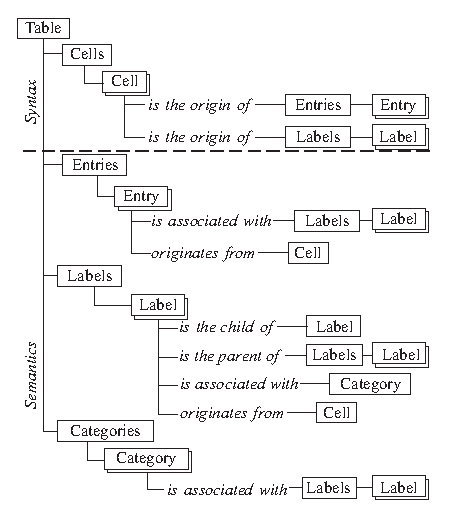
\includegraphics[width=0.85\linewidth]{tom}
%\end{figure}
\end{columns}
\end{frame}


\begin{frame}
\frametitle{CRL Grammar}
%\begin{figure}
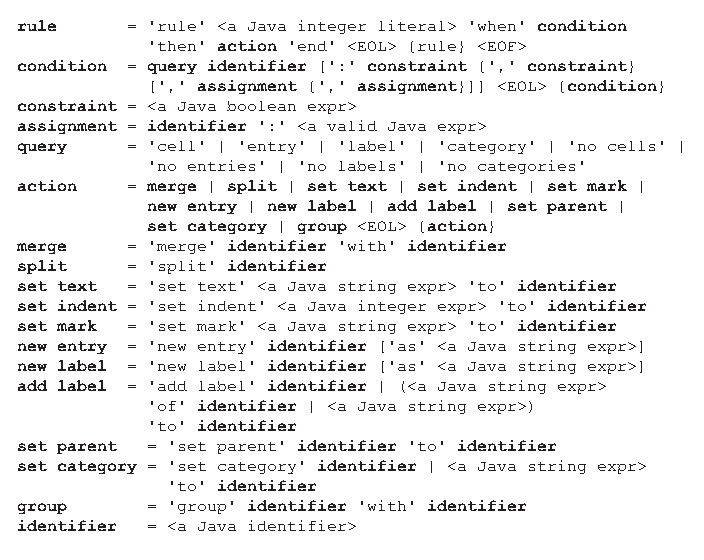
\includegraphics[width=0.75\linewidth]{BNF}
%\end{figure}
\end{frame}

\subsection{Cell Cleansing}
\begin{frame}[fragile]
\frametitle{Cell Cleansing}
The actions correct an inaccurate layout and content of a hand-coded table
\begin{itemize}
	\item \alert{<merge>} combines two adjacent cells when they share one border
	\item \alert{<split>} divides a merged cell that spans $n$-tiles (row-column intersections) into $n$-cells
	\item \alert{<set text>} modifies a textual content of a cell
	\item \alert{<set indent>} modifies a text indentation of a cell
\end{itemize}
\footnotesize{
\begin{example}
\begin{alltt}
\textbf{when}
  \textbf{cell} corner: cl == 1, rt == 1, blank
  \textbf{cell} c: cl > corner.cr, rt > corner.rb
\textbf{then}
  \textbf{split} c
\end{alltt}
\end{example}
}
\end{frame}

% \subsection{Role Analysis}

\begin{frame}[fragile]
\frametitle{Role Analysis}
The actions recover entries and labels as functional data items presented in a table
\begin{itemize}
	\item \alert{<set mark>} annotates a cell with a user-defined tag that can be used in subsequent table analysis
	\item \alert{<new entry>} (\alert{<new label>}) creates an entry (label) from a cell content with the use of an optional string processing
\end{itemize}
\footnotesize{
\begin{example}
\begin{alltt}
\textbf{when}
  \textbf{cell} corner: cl == 1, rt == 1, blank
  \textbf{cell} c: cl > corner.cr, rt > corner.rb
\textbf{then}
  \textbf{new entry} c
\end{alltt}
\end{example}
}
\end{frame}

% \subsection{Structural Analysis}


\begin{frame}[fragile]
\frametitle{Structural Analysis}
The actions recover pairs of two kinds: entry-label and label-label
\begin{itemize}
	\item \alert{<add label>} associates an entry with a label
	\item \alert{<set parent>} binds two labels as a parent and its child
\end{itemize}
\footnotesize{
\begin{example}
\begin{alltt}
\textbf{when}
  \textbf{cell} c1: cl == 1
  \textbf{cell} c2: cl == 1, rt > c1.rt, indent == c1.indent + 2
  \textbf{no cells}: cl == 1, rt > $c1.rt, rt < $c2.rt, indent == $c1.indent
\textbf{then}
  \textbf{set parent} c1.label \textbf{to} c2.label
\end{alltt}
\end{example}
}
\end{frame}


% \subsection{Interpretation}

\begin{frame}[fragile]
\frametitle{Interpretation}
The actions serve to recover label-category pairs
\begin{itemize}
	\item \alert{<set category>} associates a label with a category
	\item \alert{<group>} places two labels to one group that can be considered as an undefined category
\end{itemize}
\footnotesize{
\begin{example}
\begin{alltt}
\textbf{when}
  \textbf{label} l1: cell.mark == "stub"
  \textbf{label} l2: cell.mark == "stub", cell.rt == l1.cell.rt
\textbf{then}
  \textbf{group} l1 \textbf{with} l2
\end{alltt}
\end{example}
}
\end{frame}
% \subsection{Illustrative Example}

\begin{frame}
\frametitle{Illustrative Example}
\scriptsize{The transformation of arbitrary tables with the same layout features (\textit{a} and \textit{c}) to their canonicalized versions (\textit{b} and \textit{d})}
%\begin{figure}
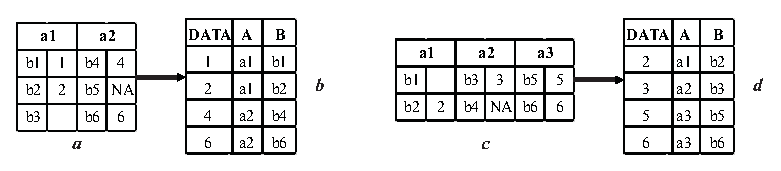
\includegraphics[width=0.7\linewidth]{illustrative_example}
%\end{figure}
\scriptsize{The ruleset for the cell cleansing (\textit{a}), role analysis (\textit{b}, \textit{c}), structural analysis (\textit{d}, \textit{e}), and interpretation (\textit{f}, \textit{g})}
%\begin{figure}
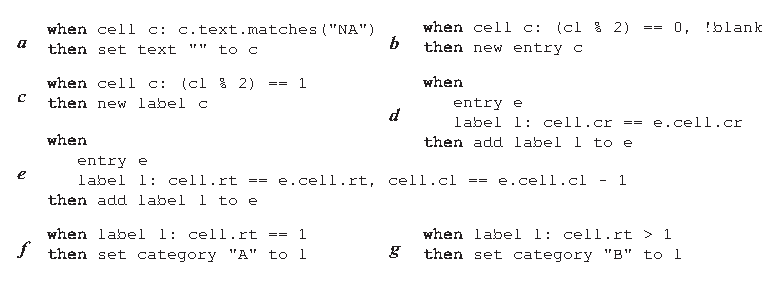
\includegraphics[width=0.75\linewidth]{illustrative_example_rules}
%\end{figure}
\tiny{This example is reproducible at \url{https://codeocean.com/capsule/5326436}}
\end{frame}

% \section{Software Platform}

% \subsection{Architecture}

\begin{frame}
\frametitle{Architecture}
%\begin{figure}
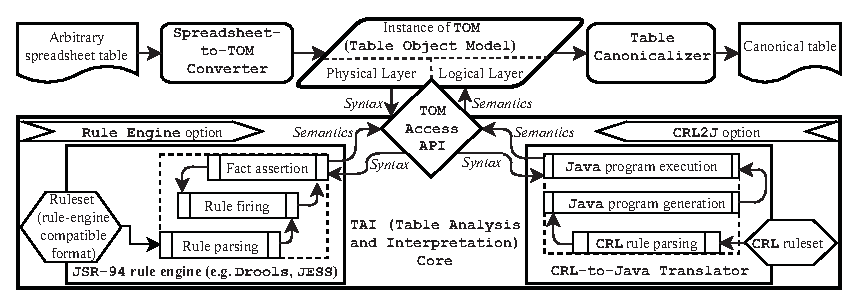
\includegraphics[width=1.0\linewidth]{architecture}
%\end{figure}
\hspace*{\fill} \textbf{Two options are provided} \hspace*{\fill}
\begin{columns}
\column{.5\textwidth}
\begin{block}{\small Rule Engine option}
\small Executing a ruleset in an appropriate format with a JSR-94 compatible rule engine (e.g. Drools, Jess)
\end{block}
\column{.4\textwidth}
\begin{block}{\small CRL2J option}
\small Translating a ruleset expressed in CRL to an executable Java program
\end{block}
\end{columns}
\end{frame}



%\subsection{CRL2J Translation}

\begin{frame}
\frametitle{CRL2J Translation}
\begin{columns}[t]
\column{.55\textwidth}
\small Workflow for generating a Maven-project of a spreadsheet data transformation program
\begin{figure}
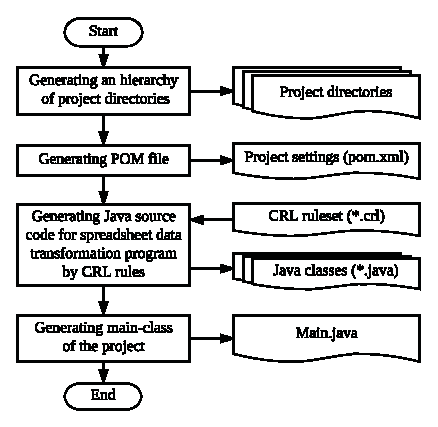
\includegraphics[width=0.95\linewidth]{crl2j_wf_part1}
\end{figure}

\column{.05\textwidth}
\\~\\

\column{.4\textwidth}
\small Workflow for translating a CRL ruleset to Java source code
\begin{figure}
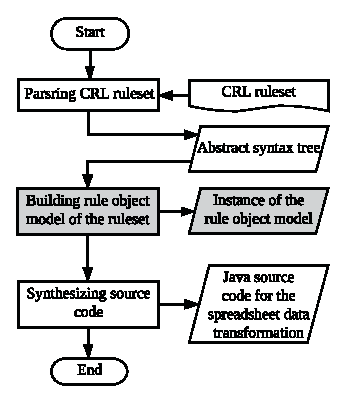
\includegraphics[width=0.95\linewidth]{crl2j_wf_part2}
\end{figure}
\end{columns}
\end{frame}

\begin{frame}
\frametitle{CRL2J Translation}

\begin{columns}
\column{.3\textwidth}
\small{\centerline{In the Workflow}}

\begin{figure}
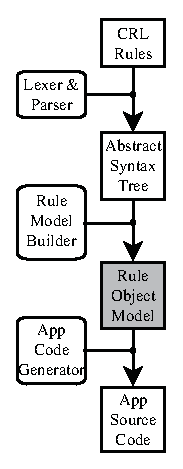
\includegraphics[width=0.65\linewidth]{rom_in_wf.eps}
\end{figure}

\column{.7\textwidth}
\small{\centerline{Rule Object Model}}

\begin{figure}
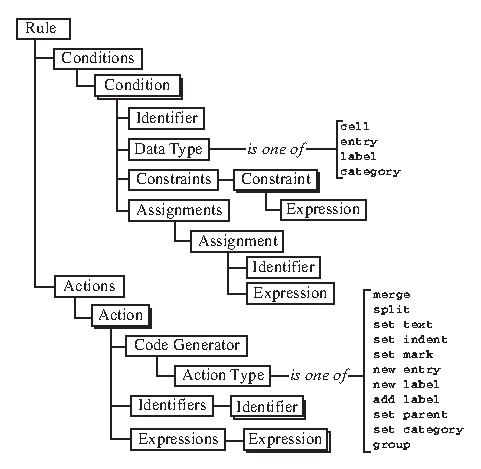
\includegraphics[width=0.8\linewidth]{rulemodel}
\end{figure}
\end{columns}

\end{frame}

\begin{frame}[fragile] % Need to use the fragile option when verbatim is used in the slide
\frametitle{CRL2J Translation}

\footnotesize{
\begin{example}[Source Rule]
\begin{alltt}
\textbf{when}
  \textbf{cell} corner: cl == 1, rt == 1, blank
  \textbf{cell} c: cl > corner.cr, rt > corner.rb, ! marked
\textbf{then}
  \textbf{set mark} "@entry" \textbf{to} c
  \textbf{new entry} c
\end{alltt}
\end{example}
}
\footnotesize{
\begin{example}[Fragment of the Generated Java Code]
\begin{alltt}
...
Iterator<CCell> iterator1 = getTable().getCells();
\textbf{while} (iterator1.hasNext()) \{
  corner = iterator1.next();
  \textbf{if} ((corner.getCl() == 1) && (corner.getRt() == 1) && ...
    Iterator<CCell> iterator2 = getTable().getCells();
    \textbf{while} (iterator2.hasNext()) \{
...
\end{alltt}
\end{example}
}
\end{frame}

%------------------------------------------------

% \section{Empirical Results}

% \subsection{Performance Evaluation}

\begin{frame}
\frametitle{Performance Evaluation}
\small{The results of the transformation of 200 tables of Troy200 dataset}
\footnotesize{
\begin{table}
		\centering
		    \bgroup
        \def\arraystretch{1.5}
				\begin{tabular}{|l|c|c|c|c|}
						\hline
														& \multicolumn{2}{|c|}{Role analysis} & \multicolumn{2}{|c|}{Structural analysis} \\
														\cline{2-5}
														& \multicolumn{4}{|c|}{Type of instances} \\
														\cline{2-5}
			            Metrics   & entries                      & labels                     & entry-label pairs            & label-label pairs  \\
			      \hline
			            Recall    & 0.9813 $\frac{16602}{16918}$ & 0.9965 $\frac{4842}{4859}$ & 0.9773 $\frac{34270}{35066}$ & 0.9389 $\frac{1951}{2078}$ \\
			            Precision & 0.9996 $\frac{16602}{16609}$ & 0.9364 $\frac{4842}{5171}$ & 0.9965 $\frac{34270}{34389}$ & 0.9784 $\frac{1951}{1994}$ \\
									$F$-score & 0.9904                       & 0.9655                     & 0.9868                       & 0.9582                     \\
			      \hline
		    \end{tabular}
				\egroup
\end{table}
}
\begin{block}{\small Metrics}
\footnotesize{
\begin{equation*}
\begin{aligned}[c]
\text{recall} = \frac{\left|R \cap S\right|}{\left|S\right|}
\end{aligned}
\quad
\begin{aligned}[c]
\text{precision} = \frac{\left|R \cap S\right|}{\left|R\right|}
\end{aligned}
\end{equation*}
}
\scriptsize{\centerline{$S$ is a set of instances in a source table, $R$ is a set of instances in its canonical form}}
\end{block}
\tiny All data and steps to reproduce the results are available at \url{http://dx.doi.org/10.17632/ydcr7mcrtp.5}
\end{frame}

\begin{frame}
\frametitle{Performance Evaluation}
\small{The comparison of the running time by using TabbyXL with three different options for transforming 200 tables of Troy200 dataset \cite{Nagy2016}}
\begin{table}
		\centering
		    \bgroup
        \def\arraystretch{1.5}
				\begin{tabular}{|l|c|c|c|}
						\hline
									Running time of             & CRL2J   & Drools  & Jess     \\
						\hline
									Ruleset preparation ($t_1$) & 2108* ms & $1711^\dagger$ ms & $432^\dagger$  ms \\
                  Ruleset execution ($t_2$)   & 367** ms & $1974^\ddagger$ ms & $4149^\ddagger$ ms \\
			      \hline
		    \end{tabular}
				\egroup
\end{table}
\scriptsize{
* $t_1$ --- a time of parsing and compiling the original ruleset into a Java program \\
** $t_2$ --- a time of executing the generated Java program
\\~\\
$^\dagger$ $t_1$ --- a time of parsing the original ruleset and adding the result into a rule engine session \\
$^\ddagger$ $t_2$ --- a time of asserting facts into the working memory and matching rules against the facts
\\~\\
For testing, we used 3.2 GHz 4-core CPU
}
\end{frame}

% \subsection{Comparison with Others}

\begin{frame}
\frametitle{Comparison with Others}

\small{
\begin{block}{Role Analysis}
\begin{itemize}
\item \emph{Contest task}: The segmentation of a table into typical functional cell regions
\item \emph{Testing dataset}: Troy200  \cite{Nagy2016}
\item \emph{Contestant}: MIPS (TANGO) \cite{Embley2016}
\item \emph{Accuracy}: MIPS (TANGO) --- \textbf{0.9899} vs. TabbyXL --- \textbf{0.9950}
\end{itemize}
\end{block}

\begin{block}{Structural Analysis}
\begin{itemize}
	\item \emph{Contest task}: The extraction of header hierarchies from tables
	\item \emph{Testing dataset}: A random subset of SAUS\footnote{\url{http://dbgroup.eecs.umich.edu/project/sheets/datasets.html}}
	\item \emph{Contestant}: Senbazuru \cite{Chen2014}
	\item $F$\emph{-score}: Senbazuru --- \textbf{0.8860} vs. TabbyXL --- \textbf{0.8657}
\end{itemize}
\end{block}
}
\end{frame}

\section{Application Experience}

\begin{frame}
\frametitle{Application Experience}
Populating a web-based statistical atlas of the Irkutsk region --- (\textit{b}) via extracting data from government statistical reports --- (\textit{a})
\begin{figure}
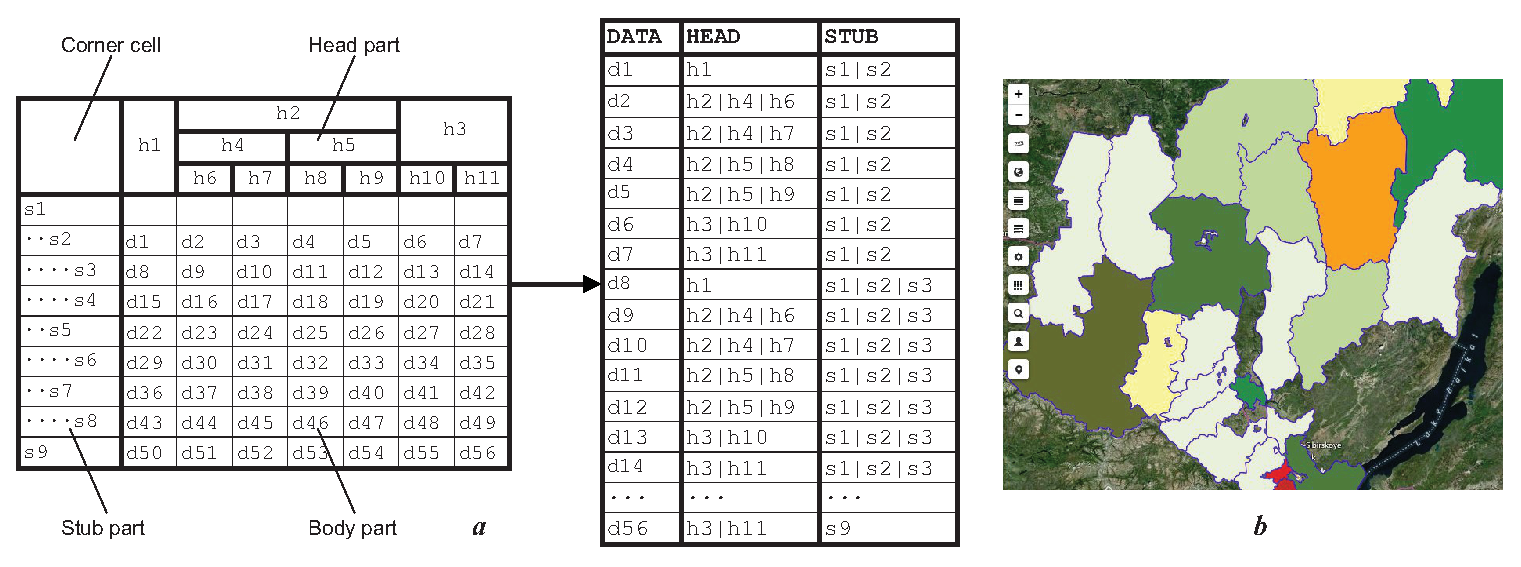
\includegraphics[width=1\linewidth]{application1}
\end{figure}
\tiny{The more detail can be found at \url{https://github.com/tabbydoc/tabbyxl/wiki/statistical-atlas}}
\end{frame}

\begin{frame}
\frametitle{Application Experience}
Generating conceptual models --- (\textit{b}) from arbitrary tables presented in industrial safety inspection reports --- (\textit{a})
\begin{figure}
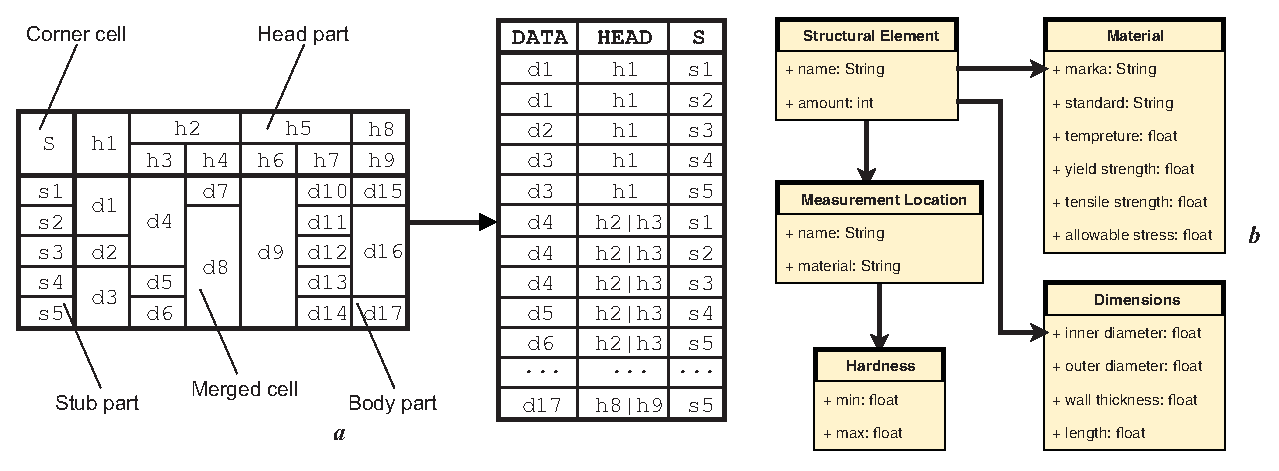
\includegraphics[width=1\linewidth]{application2}
\end{figure}
\tiny{The more detail can be found at \url{https://github.com/tabbydoc/tabbyxl/wiki/industrial-safety-inspection}}
\end{frame}

% \section{Conclusions \& Further Work}

\begin{frame}
\frametitle{Conclusions \& Further Work}

\begin{itemize}
\item Impact on software development for spreadsheet data management
\begin{itemize}
\item Table object model associating functional roles with data items
\item Table analysis and interpretation driven by user-defined rules
\item Formulated actions to recover missing semantics of arbitrary tables
\item Translation of rules to executable spreadsheet transformation programs
\end{itemize}
\medskip
\item Limitations
\begin{itemize}
\item The inaccurate cell structure prevents the table analysis
\item The very limited interpretation (without external vocabularies)
\end{itemize}
\medskip
\item Further work
\begin{itemize}
\item Rearrangement of cell structure by using visual (human-readable) cells
\item Detecting derived data by spreadsheet formulas
\item Enriching the table analysis by named entity recognition
\item Linking extracted data items with LOD cloud
\end{itemize}
\end{itemize}

\end{frame}

\section{References}

\begin{frame}[allowframebreaks]
\frametitle{References}
\tiny
\bibliographystyle{apalike}
\bibliography{mybibfile}
\end{frame}

\begin{frame}
\Huge{\centerline{Thanks}}
\bigskip
\footnotesize{\centerline{Read more about the project at}}
\scriptsize{\centerline{\url{http://td.icc.ru}}}

\bigskip
\footnotesize{\centerline{The project source code is available at}}
\scriptsize{\centerline{\url{https://github.com/tabbydoc/tabbyxl}}}
\end{frame}





% ----------------------------------------------------------------------------------

\begin{frame}
  \begin{center}
  \Large Thanks for Your interest to our project!
\end{center}
\end{frame}

\begin{frame}[fragile]
  \frametitle{Rapidminer module}
\begin{minted}[fontsize=\tiny]{cpp}
vector<string> AlignCommand::setParameters(){ // PART OF MODULE SOURCE
try {
  CommandParameter ptemplate("reference", "InputTypes", "", "", "none", "none", "none","",false,true,true); parameters.push_back(ptemplate);
  CommandParameter pcandidate("fasta", "InputTypes", "", "", "none", "none", "none","fasta-alignreport-accnos",false,true,true); parameters.push_back(pcandidate);
  CommandParameter psearch("search", "Multiple", "kmer-blast-suffix", "kmer", "", "", "","",false,false,true); parameters.push_back(psearch);
  CommandParameter pksize("ksize", "Number", "", "8", "", "", "","",false,false); parameters.push_back(pksize);
  CommandParameter pmatch("match", "Number", "", "1.0", "", "", "","",false,false); parameters.push_back(pmatch);
// . . . . . . .
\end{minted}
\begin{minted}[fontsize=\tiny]{java}
package com.rapidminer.ngs.operator; // GENERATED JAVA MODULE
// imports

class MothurChimeraCcodeOperator extends MothurGeneratedOperator {
  private InputPort fastaInPort = getInputPorts().createPort("fasta");
  private InputPort referenceInPort = getInputPorts().createPort("reference");
  private OutputPort chimeraOutPort = getOutputPorts().createPort("chimera");
  private OutputPort mapinfoOutPort = getOutputPorts().createPort("mapinfo");
  private OutputPort accnosOutPort = getOutputPorts().createPort("accnos");

  public MothurChimeraCcodeOperator (OperatorDescription description) {
    super(description);
  }
  @Override
  public void doWork() throws OperatorException {
    super();
    // . . . . . .
  }
  @Override
  public List<ParameterType> getParameterTypes() {
    super();
        // . . . . . .
  }
  @Override
  public String getOutputPattern(String type) {
    if (type=="chimera") return "[filename],[tag],ccode.chimeras-[filename],ccode.chimeras";
    if (type=="mapinfo") return "[filename],mapinfo";
    if (type=="accnos") return "[filename],[tag],ccode.accnos-[filename],ccode.accnos";
    return super.getOutputPattern(type);
  }
}
\end{minted}
\end{frame}

\begin{frame}[fragile]
  \frametitle{RDF (TTL) representation and ad its query object}
\begin{multicols}{2}
\begin{minted}[fontsize=\tiny]{turtle}
@prefix xml: <http://www.w3.org/XML/1998/namespace> .
@prefix xsd: <http://www.w3.org/2001/XMLSchema#> .
ngsp:spec a ngsp:Specification ;
    ngsp:module mothur:NoCommand,
        mothur:align-check,
        mothur:align-seqs,
# . . . . .
mothur:align-check a ngsp:Module ;
    ngsp:outputPattern [ a cnt:Chars ;
            ngsp:parameterName "type" ;
            ngsp:pattern [ ngsp:patternString
                    "[filename],align.check" ;
                    dc:identifier "aligncheck" ] ;
            cnt:chars # . . . .
# . . . . .
mothur:align-check-idir-parameter a ngsp:Parameter ;
    ngsp:important false ;
    ngsp:multipleSelectionAllowed false ;
    ngsp:optionsDefault "" ;
    ngsp:required false ;
    ngsp:type mothur:String ;
    dc:title "inputdir" .

mothur:align-check-map-parameter a ngsp:Parameter ;
    ngsp:important true ;
    ngsp:multipleSelectionAllowed false ;
    ngsp:optionsDefault "" ;
    ngsp:required true ;
    ngsp:type mothur:InputTypes ;
    dc:title "map" .

mothur:align-check-name-parameter a ngsp:Parameter ;
    ngsp:chooseOnlyOneGroup "namecount" ;
    ngsp:important false ;
    ngsp:multipleSelectionAllowed false ;
# . . . . .
\end{minted}
\begin{minted}[fontsize=\tiny]{logtalk}
:- object(queryparam(_RDF,_Parameter),
          extends(ngsquerybase)).

:- public(type/1).
type(Type) :-
    ::attr(type, Type).
:- public(name/1).
name(Name) :- ::attr(dc:title, literal(Name)).
:- public(options/1).
options(Value):- ::attr(options, Value).
:- public(options_default/1).
options_default(Value):-
    ::attr(optionsDefault, Value).
% . . . . . . . .
:- public(multiple_selection_allowed/0).
multiple_selection_allowed:-
    ::bool_attr(multipleSelectionAllowed).
:- public(required/0).
required:-
    ::bool_attr(required).
:- public(important/0).
important:-
    ::bool_attr(important).
:- protected(attr/2).
attr(NS:Name, Value):-
    ::ngs(RDF),
    ::second(Parameter),
    rdf_db::rdf_global_object(Value, V),
    RDF::rdf(Parameter, NS:Name, V).
attr(Name, Value):-
    \+ Name=_:_,!,
    ::ngs(RDF),
    ::second(Parameter),
    rdf_db::rdf_global_id(Value, V),
    RDF::rdf(Parameter, ngsp:Name, V).
% . . . . .
:- end_object.

\end{minted}
\end{multicols}
\end{frame}


\end{document}

%%% Local Variables:
%%% mode: latex
%%% TeX-master: t
%%% End:
